
\documentclass{beamer}
\usepackage{amsmath,amssymb,amsfonts,mathrsfs,accents}
\usepackage{array}
\usepackage{graphicx}
\usepackage{caption}
\usepackage{subcaption}
\usepackage[utf8]{inputenc}
\usetheme{Madrid}
\usecolortheme{default}
\usepackage{blindtext}
\usepackage{hyperref}
\setbeamertemplate{caption}[numbered]
\usepackage{listings}
\renewcommand{\lstlistingname}{Model}
\lstset{frame=none, framexleftmargin=4pt, framexrightmargin=4pt, backgroundcolor=\color{code_bg}, basicstyle=\footnotesize\ttfamily, tabsize=2}


%-----------------------------------------------------------------------------------%

\begin{document}
\title{Green transition in the power sector: a model of technology adoption}
\author{Maija Kaartinen and Alireza Azampour}
\date{\today}
\maketitle
	
%----------------------------------------------------------------------------------

\begin{frame}{Power sector investment dynamics}

\begin{itemize}
 \item Electricity and heat production accounted for $33\%$ of global greenhouse gas emissions in 2020
 \item Climate policies impact firms' technology choice via
 \begin{itemize}
     \item Operation costs: carbon taxes
     \item Fixed costs: installation subsidies, innovation
 \end{itemize}
\item Firms' investment decisions have large policy implications
\item The age, type, and quality of initial technological capital likely plays a role in this
\end{itemize}
\end{frame}
%%%%%%%%%%%%%%%
\begin{frame}{US power sector: two transitions}


\begin{table}
\centering
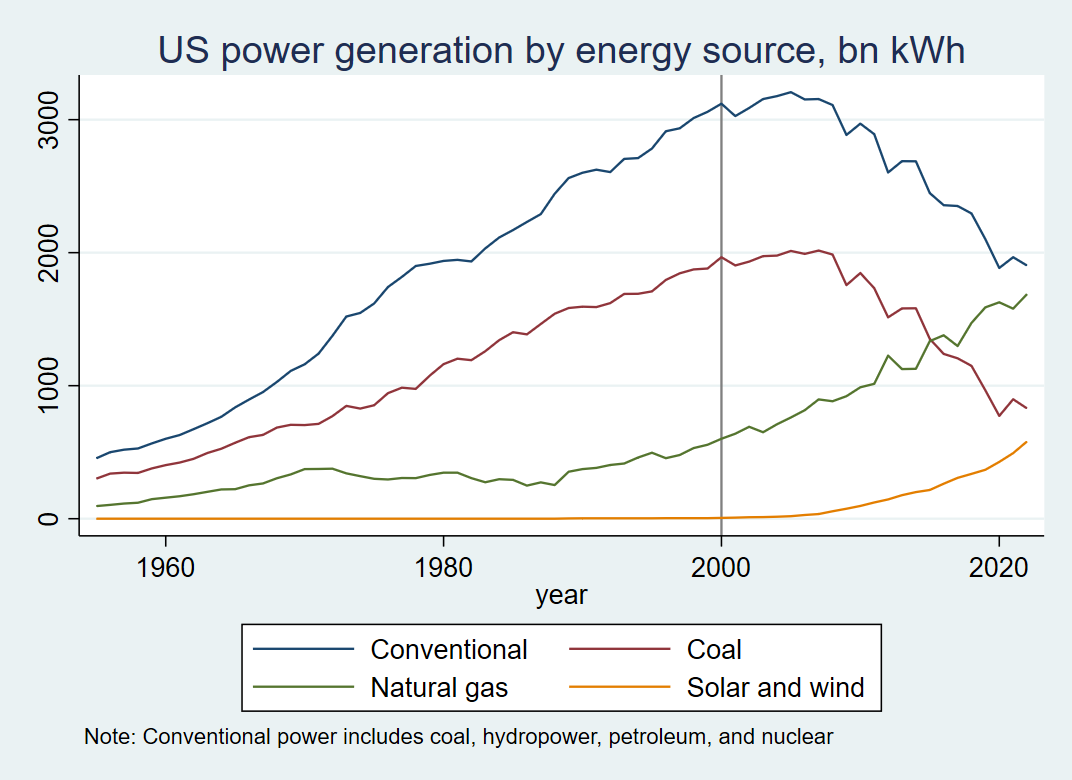
\includegraphics[scale=0.25]{US_powergeneration_trends.png}
\end{table}
    
\end{frame}
%%%%%%%%%%%%%%%
\begin{frame}{Research question}
\large 
\begin{center}
    "How do power sector firms make investment choices between different technology types, and how do these choices depend in their initial capital?"\\\\
\hfill \break
"How do these firm-level dynamics impact the efficiency of power sector subsidies and carbon pricing?"

\end{center}

    
\end{frame}
%%%%%%%%%%%%%%%
\begin{frame}{Outline of the project}

\begin{itemize}
    \item We present a model of heterogeneous power generators 
    \item Data on US power generators is used to test the implications of the model
    \item The model is calibrated to match the US power sector transitions towards 1) natural gas and 2) wind and solar power
    \item Counterfactual analysis is used to test the implications of IRA installations subsidies and other policies
    \item Shocks to relative input prices are used to test whether the model supports a CES energy production function
    \item Objective: a micro-founded alternative to conventional engineering and CES models, which can be used to assess the importance of fixed costs for power sector transition
\end{itemize}

    
\end{frame}
%%%%%%%%%%%%%%%

\begin{frame}{The model: generator technology choice, entry and exit}

\begin{itemize}
 \item Generators produce electricity in a perfectly competitive market using a fuel input
 \item They belong to one of two technology types: old or new
 \item Generators' competitiveness depends on the age and efficiency of their technology
 \item In each period, a generator can choose to pay an adoption cost and draw a new technological efficiency value. It exits if its present value goes to zero
 \item Potential entrants can pay an entry cost and draw an initial efficiency value $a_{i,0}$
 \item Perfect competition implies that generator decisions are independent of which firm owns them
\end{itemize}
    
\end{frame}
%%%%%%%%%%%%%%%
\begin{frame}{The model: market structure}
\begin{itemize}
 \item Generators using the old and new technology use the fuel input $e_i^o$ or $e_i^n$ at prices $p_i^o$ or $p_i^n$, respectively
  \item Both types sell electricity at the price $p_E$
 \item Productivities are drawn from an exponential distribution with mean $\overline{a}^o$ or $\overline{a}^n$: productivity growth is exogenous
 \item The two types pay different technology adoption costs $c_a^o$ and $c_a^n$ and operation costs $c_f^o$ and $c_f^n$
 \item Electricity demand is given by: $\ln(d) = d_0-\varepsilon\ln(p_E)$
 \item Fuel input supply is given by:  $e_i(p_{e,i}) = e_{0,i}p_{e,i}^{\epsilon_{i}}$

\end{itemize}
    
\end{frame}
%%%%%%%%%%%%%%%
\begin{frame}{The model: generator's problem}
\begin{align*} 
    v(a_{i},t) &= \max_{e_i,aot=\{0,1\}} p_E\frac{a_{i}^{1+\gamma t}}{(1+g_a)^t} e_i^\alpha -p_e e_i-c_f\\ 
    &+\beta \big(\mathbf{1}_{\{aot =0\}} \mathbb{E}[v(a_{i},t+1)] + \mathbf{1}_{\{aot =1\}}[ \mathbb{E}[v(a_{i}',t-\tau)]-c_a]\big)
\end{align*}
\begin{itemize}
 \item $E_i =\frac{a_{i}^{1+\gamma t}}{(1+g_a)^t} e_i^\alpha$ is the electricity production of the generator where $\frac{a_{i}^{1+\gamma t}}{(1+g_a)^t}$ is its efficiency relative to the market\\
    \item Technology draws follow $a'_i\sim \rho a_i + (1-\rho)\epsilon_i$ where $\epsilon_i$ follows an $i.i.d$ exponential distribution
    \item $p_E$ and $p_e$ are the electricity and fuel input prices
    \item $g_a$ is the rate at which a generator's relative efficiency declines
    \item $c_a$ is the cost of adoption and  $c_f$ is the fixed cost of operation.
\end{itemize}
    
\end{frame}
%%%%%%%%%%%%%%%
\begin{frame}{The model: entry and exit}
\begin{itemize}
    \item The value of entry is given by: 
    \begin{equation*}
    \begin{aligned} 
    E[v(a_{i,0},0)]-c_{e}=\\\int \big\{ p_Ea_{i,0} e_i^\alpha -p_e e_i+E[v(a_{i,0},1)] \big\} dD(a_{i,0})-c_{e}
\end{aligned}
    \end{equation*}
    
where $c_{e}$ is the entry cost and $a_{i,0}$ is drawn from the exponential distribution
\hfill \break
    \item If $v<0$ the generator exits\\
    \item $\kappa$ is the exogenous exit rate
\end{itemize}
    
\end{frame}
%%%%%%%%%%%%%%%
\begin{frame}{Equilibrium}
    \begin{itemize}
        \item The Equilibrium consists of policy function $P(a_i,t)$, a stationary distribution of generators $\Gamma$ with the measure $m_{ss}$, and an equilibrium price $p_E$ where
        \item  $P(a_i,t)$ is the answer to firms' problem at the price $p_E$
        \item The electricity market clears at the price $p_E$ 
        \item The fuel input markets clear at prices $p_e^o$ and $p_e^n$
        \item The value of entry is zero, or the the mass of generators is zero for both technology types
    \end{itemize}
\end{frame}

%%%%%%%%%%%%%%%%
\begin{frame}{Data: EIA power generator data}

\begin{itemize}
 \item EIA US power generator data from years 1991-2021
 \item The data includes utility power plants until year 2000: all power plants included thereafter. Unbalanced panel
 \item Generator data on capacity, energy sources, operating status, maintenance, first year of operation, location, owner, and power plant
 \item Plant-level data on net generation and fuel consumption
  \item The data analysis only covers generators that use a  fuel


\end{itemize}
    
\end{frame}
%%%%%%%%%%%%%%%
\begin{frame}{Variables constructed for analysis}

 \begin{itemize}
     \item Efficiency: fuel consumption per unit of net generation
     \item Efficiency update dummy: 1 when efficiency increases by 10\% or more but the ratio between capacity and generation does not change by more than 5\% (we test several thresholds)
     \item Capacity age: number of years since the latest update
 \end{itemize}

    
\end{frame}
%%%%%%%%%%%%%%%

\begin{frame}{Power plant summary statistics}
\footnotesize
\begin{table}[htbp]\centering
\footnotesize
\def\sym#1{\ifmmode^{#1}\else\(^{#1}\)\fi}
\caption{Summary statistics, All plants used in analysis}
\begin{tabular}{l*{1}{cccccc}}
\hline\hline

                    &        mean&          sd&         min&         max&           N\\
\hline
No of generators    &         3.5&         3.2&         1.0&        48.0&    84,601\\
No of energy sources used&         1.3&         0.5&         1.0&         5.0&    84,601\\
No of energy sources per generator&         1.5&         0.7&         1.0&         6.0&    84,601\\
Average generator age&        24.5&        15.4&         0.0&        96.0&    84,601\\
Summer capacity     &       241.2&       451.3&         0.0&     3,814.0&    84,570\\
Fuel efficiency     &         0.3&         0.1&         0.0&         1.0&    77,960\\
Relative efficiency &         0.9&         0.4&         0.0&         3.6&    77,960\\
Relative efficiency after latest update&         1.1&         0.4&         0.0&         3.3&    10,359\\
Share updating per year&         3.0&        17.0&         0.0&       100.0&    71,558\\
Share updating per year, unconstrained&        14.9&        35.6&         0.0&       100.0&    71,558\\
\hline\hline
\multicolumn{6}{l}{\footnotesize Note: Summary statistics over plant-year}\\
\end{tabular}
\end{table}

\footnotesize{Note: Adoption dummy defined as efficiency increase of at least 10\% with less than 5\% variation in the capacity-to-generation dummy }

    
\end{frame}
%%%%%%%%%%%%%%%
\begin{frame}{Power plant capacity age distribution}

\begin{figure}
\centering
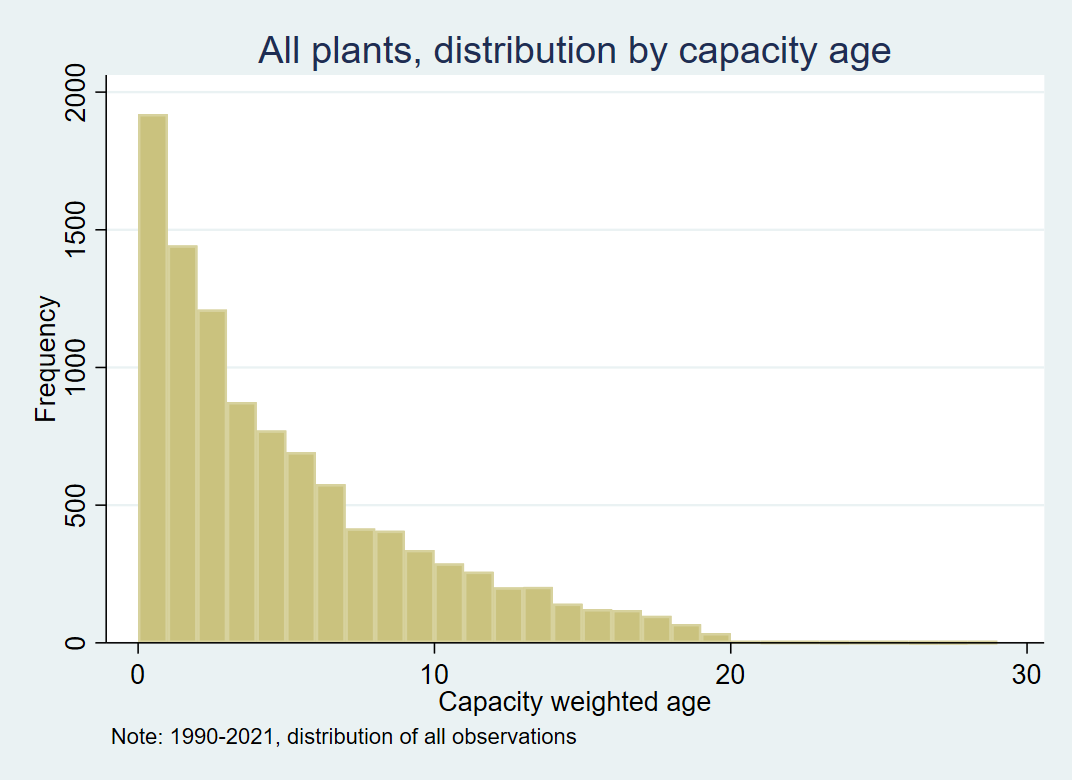
\includegraphics[scale=0.25]{EFFIC_all_capage_hist.png}
\end{figure}
\scriptsize{Note: Technological update implies an efficiency increase of at least 10 \%, with less than 5 \% variation in generator capacity-to-generation ratio}
    
\end{frame}
%%%%%%%%%%%%%%%
\begin{frame}{Power plant efficiency distribution}

\begin{figure}
\centering
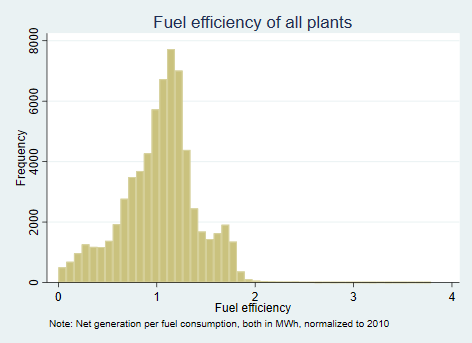
\includegraphics[scale=0.25]{EFFIC_effic_plant_norm_all_hist.png}
\end{figure}
\scriptsize{Note: Technological update implies an efficiency increase of at least 10 \%, with less than 5 \% variation in generator capacity-to-generation ratio}
    
\end{frame}
%%%%%%%%%%%%%%%
\begin{frame}{Power plant efficiency distribution, after update}

\begin{figure}
\centering
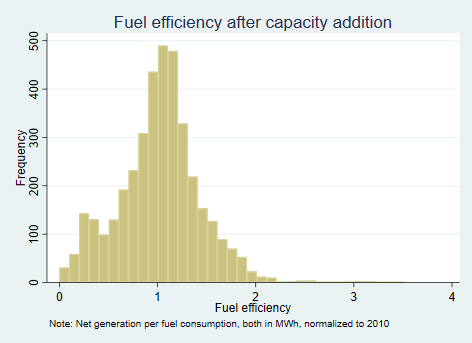
\includegraphics[scale=0.25]{EFFIC_effic_plant_new_norm_all_hist.png}
\end{figure}
\scriptsize{Note: Technological update implies an efficiency increase of at least 10 \%, with less than 5 \% variation in generator capacity-to-generation ratio}
    
\end{frame}
%%%%%%%%%%%%%%%
\begin{frame}{Model: Steady state results}
\begin{figure}
\centering
\caption{Conventional power plants: distribution before transition}
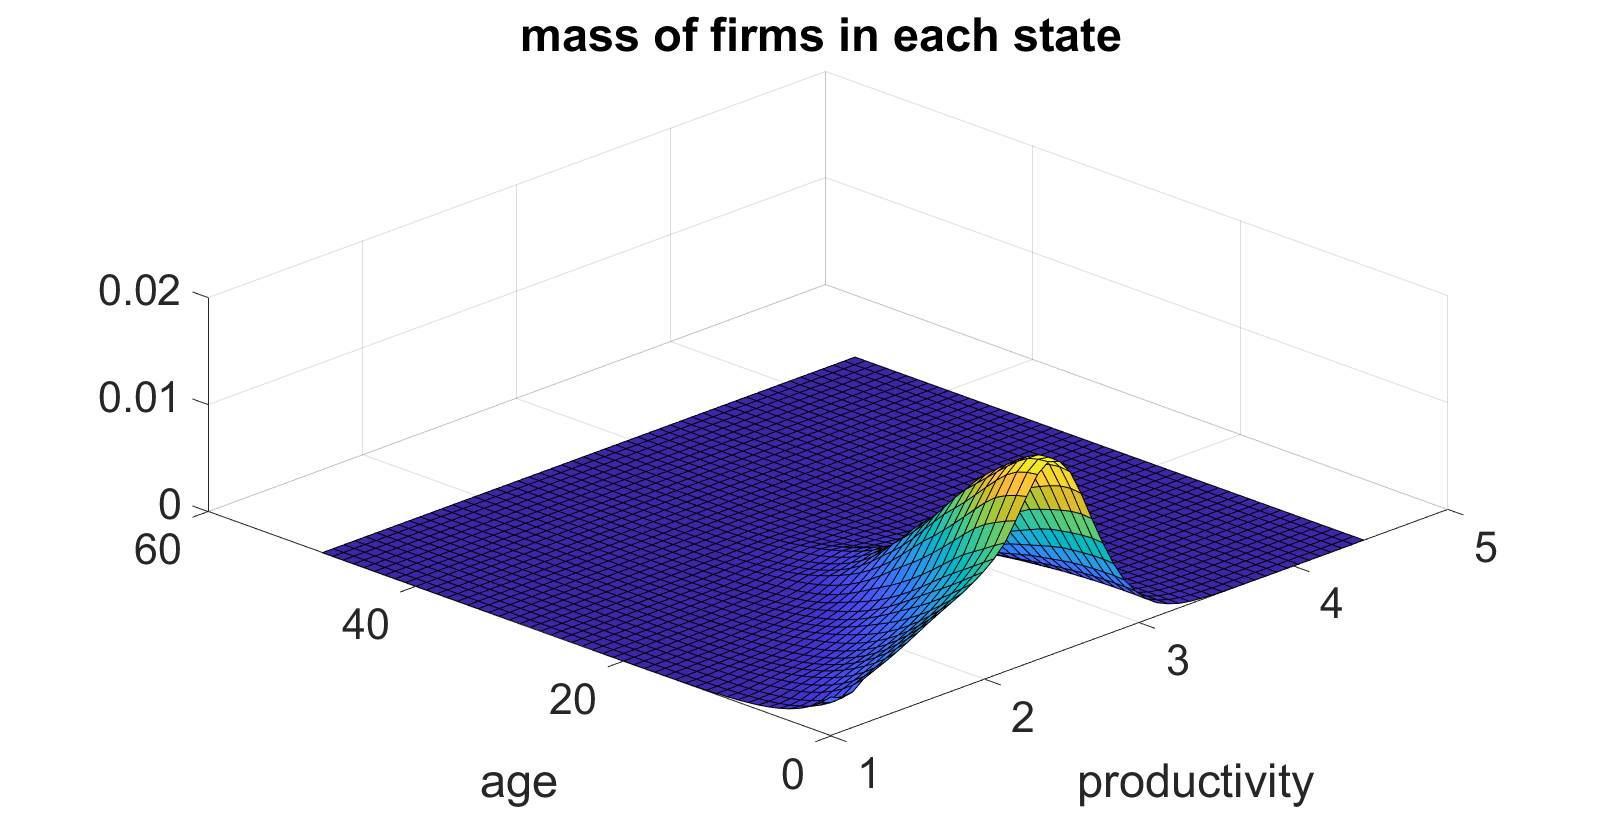
\includegraphics[scale=0.25]{dist_gas_before.png}
\end{figure}
\end{frame}

%%%%%%%%%%%%%%%%
\begin{frame}{Model: Steady state results}
\begin{figure}
\centering
\caption{Solar and wind power plants: distribution before transition}
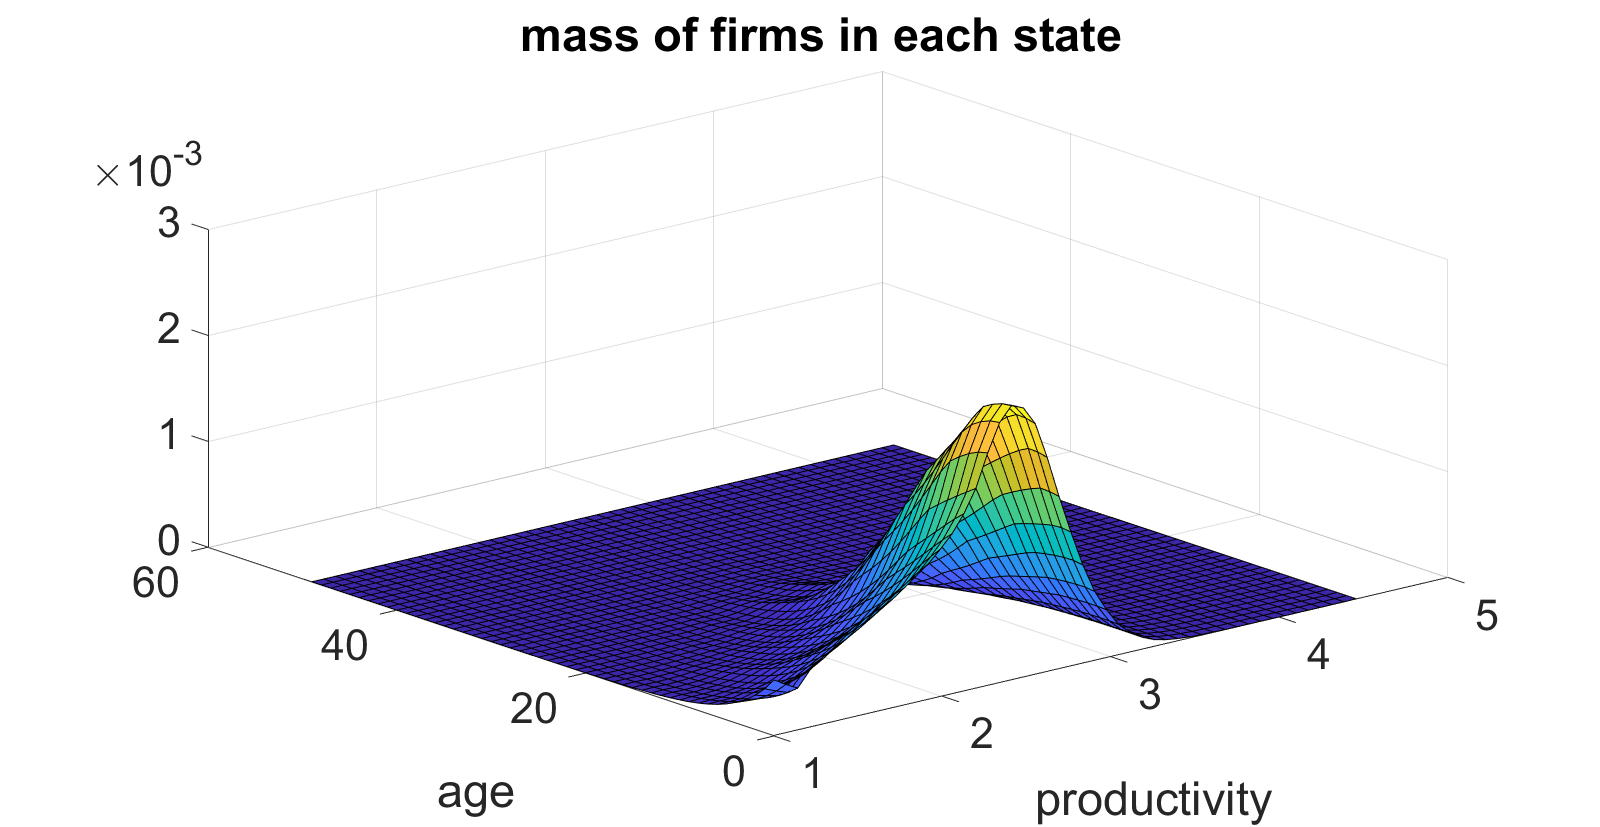
\includegraphics[scale=0.25]{dist_solar_before.png}
\end{figure}
\end{frame}

%%%%%%%%%%%%%%%%

\begin{frame}{Model: Steady state results}
\begin{figure}
\centering
\caption{Conventional power plants: probability of technology adoption before transition}
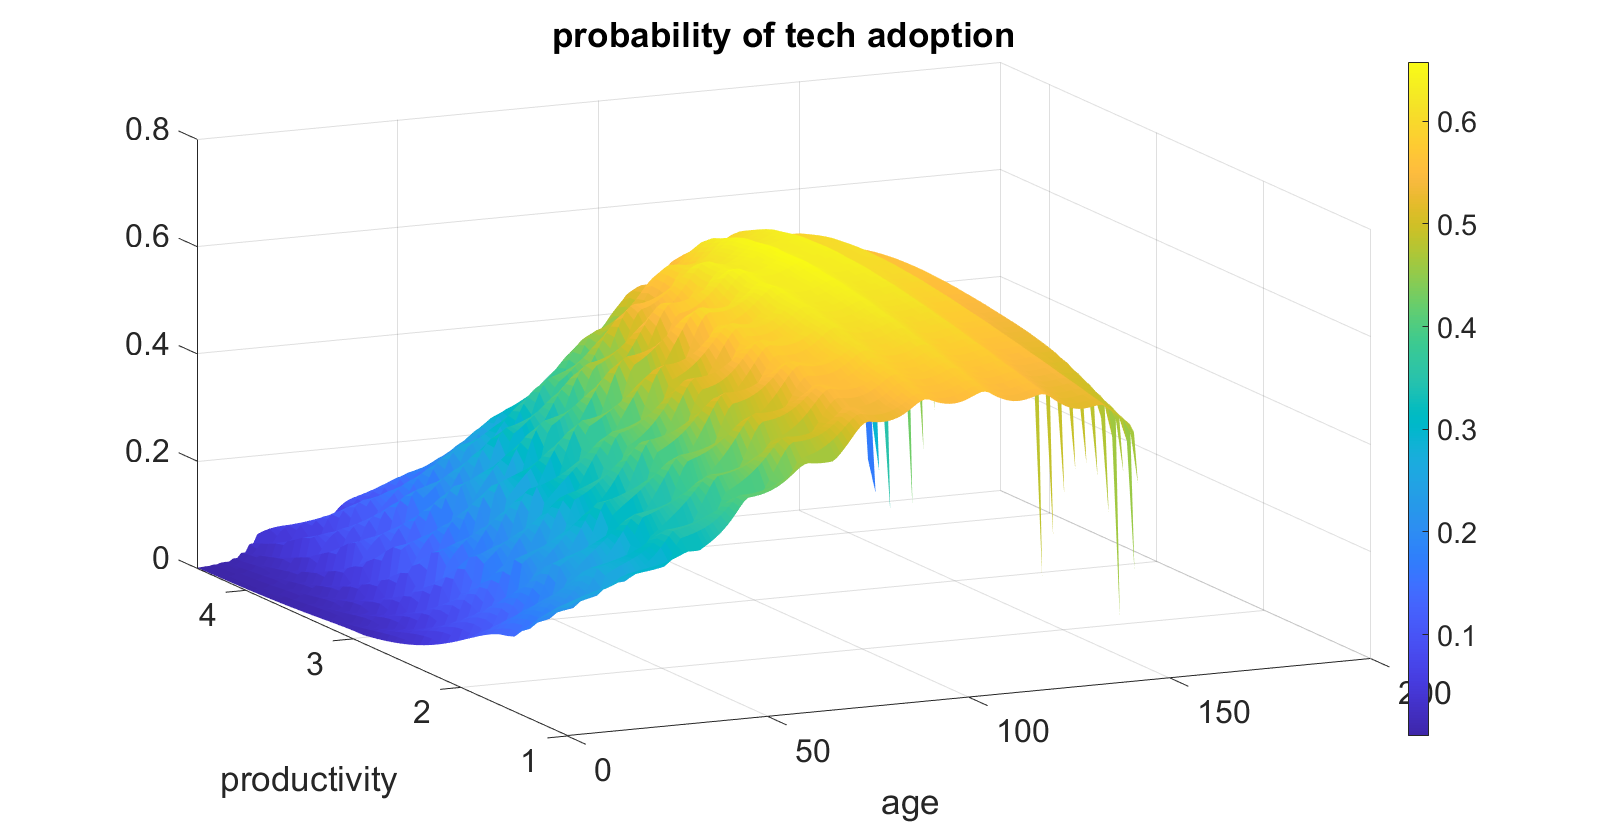
\includegraphics[scale=0.25]{prob_gas_before.png}
\end{figure}
\end{frame}

%%%%%%%%%%%%%%%%
\begin{frame}{Model: Steady state results}
\begin{figure}
\centering
\caption{Solar and wind power plants: probability of technology adoption before transition}
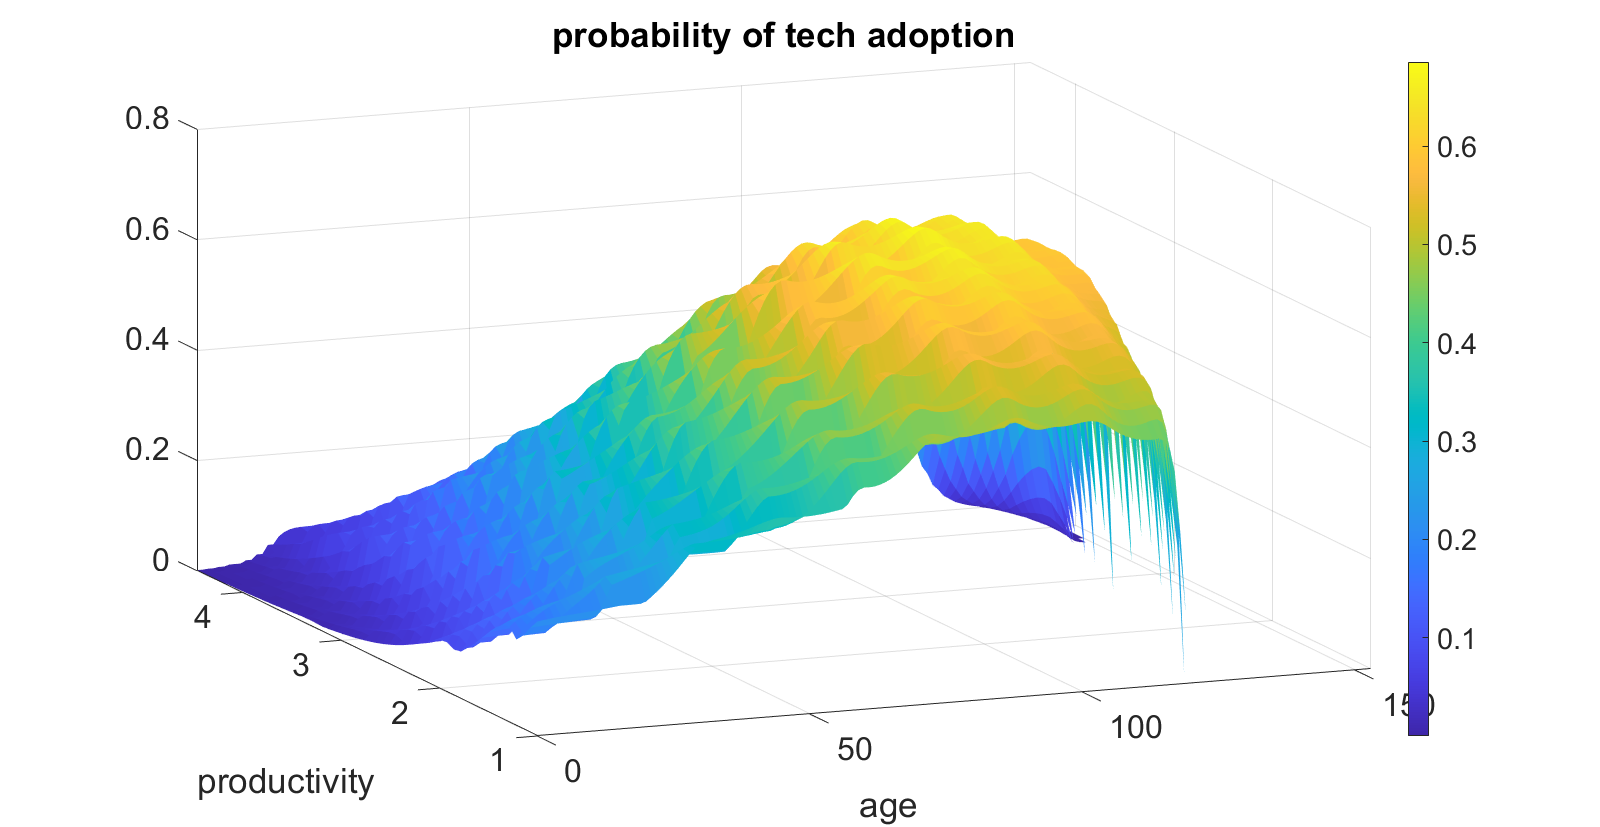
\includegraphics[scale=0.25]{prob_sola_before.png}
\end{figure}
\end{frame}

%%%%%%%%%%%%%%%%

\begin{frame}{Data: Adoption patterns}

\begin{table}
\centering
\caption{Technology adoption dummy regressed on covariates}
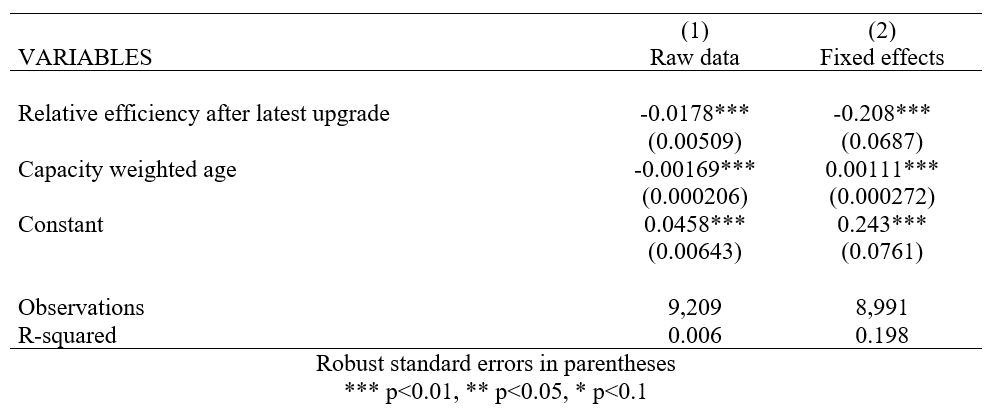
\includegraphics[scale=0.65]{Part4_1_all.png}
\end{table}
\footnotesize{Note: Adoption dummy defined as efficiency increase of at least 10\% with less than 5\% variation in the capacity-to-generation dummy }

\end{frame}
%%%%%%%%%%%%%%%%

\begin{frame}{Data: Adoption patterns}

\begin{table}
\centering
\caption{Technology adoption dummy regressed on covariates}
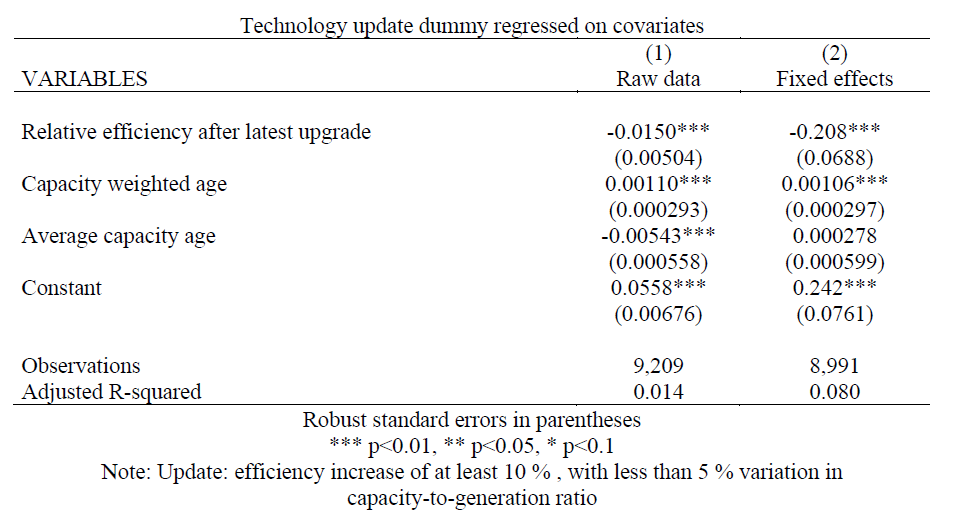
\includegraphics[scale=0.75]{Part4_durab_10_5.png}
\end{table}


\end{frame}


\begin{frame}{Calibration}
    \begin{itemize}
        \item $c_e$ will be derived from data on average construction costs
        \item $c_f$ will be calibrated to match data on average operation costs 
        \item $c_a$ will be calibrated internally, matching the share of generators updating their technology each year
        \item The distribution of $\epsilon$ and $a_0$ will be matched to generators' fuel cost efficiency distribution
        \item $\alpha$ will be matched to the aggregate ratio between input fuel and net generation
         \item $\rho$ will be calibrated equal to the autocorrelation in plant efficiency values (0.7)
        \item Exit rate will be set equal to the plant retirement rate of around 1 \%
        \item Supply and demand elasticities: from empirical estimates (Burke and Abayasekara, 2018)
    \end{itemize}
\end{frame}
%%%%%%%%%%%%%%%
\begin{frame}{Calibration: efficiency in periods between updates}
Firm decision:\\
\begin{align*} 
    v(a_{i},t) &= \max_{e_i,aot=\{0,1\}} p_E\frac{a_{i}^{1+\gamma t}}{(1+g_a)^t} e_i^\alpha -p_e e_i-c_f\\ 
    &+\beta \big(\mathbf{1}_{\{aot =0\}} \mathbb{E}[v(a_{i},t+1)] + \mathbf{1}_{\{aot =1\}}[ \mathbb{E}[v(a_{i}',t-\tau)]-c]\big)\\
\end{align*}
Between two updates the efficiency of a generator is then given by:\\
\begin{align*}
    a_{i,t} &= \frac{a_{i,t-\tau}}{(\frac{1+g_t}{a_{i,0}^\gamma})^\tau}  \rightarrow \ln a_{i,t} = \ln a_{i,t-\tau} -  \tau \ln(1+g_t) + \tau \gamma\ln a_{i,0} 
\end{align*}
    
\end{frame}

%%%%%%%%%%%%%%%

\begin{frame}{Regression results: efficiency in periods between updates}
\begin{table}
\centering
\caption{Relative efficiency in periods between updates, with the interaction between capacity age and durability}
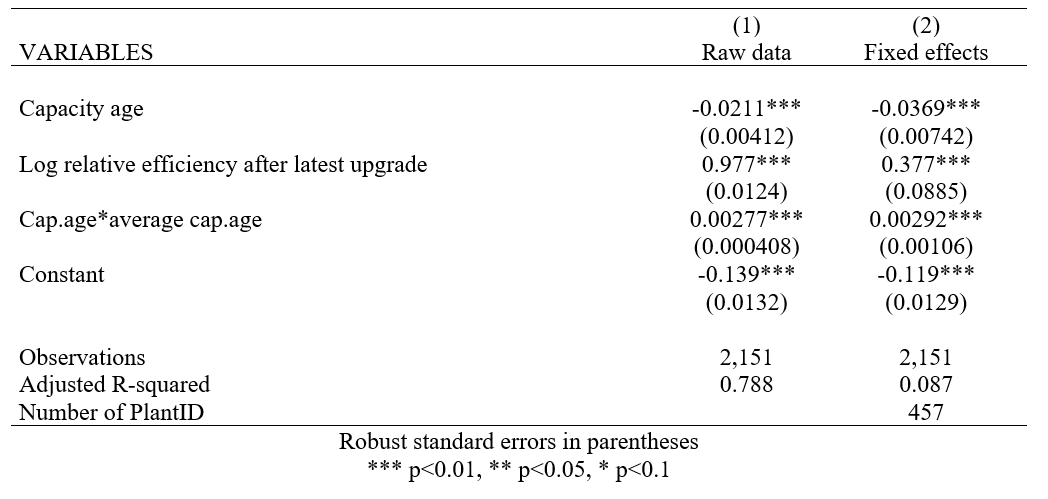
\includegraphics[scale=0.62]{5_5_effic_noupd_age_effic_LOG_capageinteract_1gen.png}
\end{table}
\scriptsize{Note: Relative efficiency denotes efficiency relative to newly updated generators. Capacity age denotes years since the latest update, defined as an efficiency increase of over 5\%}

\end{frame}

%%%%%%%%%%%%%%%

\begin{frame}{Transition 1: Conventional fuels to natural gas}

\begin{center}
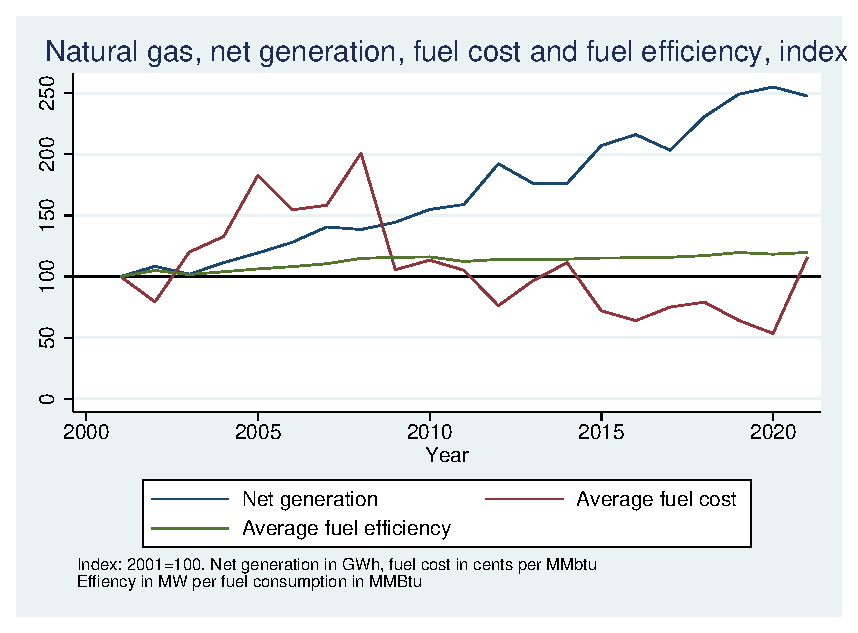
\includegraphics[scale=0.65]{NG_cost_gen_effic.eps}
\end{center}

\end{frame}
%%%%%%%%%%%%%%%
\begin{frame}{Transition 1: Conventional fuels to natural gas}

\begin{center}
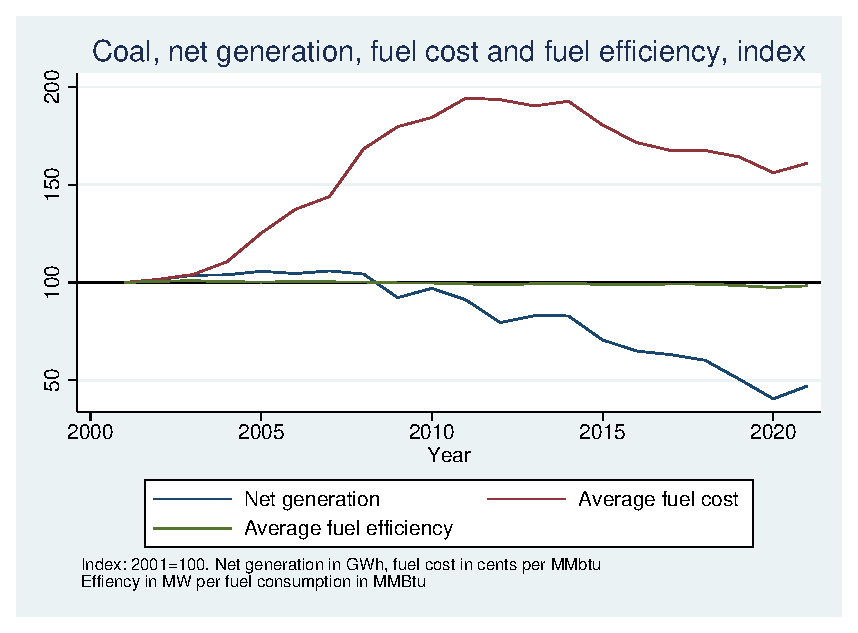
\includegraphics[scale=0.65]{Coal_cost_gen_effic.eps}
\end{center}

\end{frame}
%%%%%%%%%%%%%%%

\begin{frame}{Transition 1: Conventional fuels to natural gas}

\begin{itemize}
    \item First a shock to the efficiency distribution of natural gas generators
    \item Later a shock to its input price
\end{itemize}

    
\end{frame}

\begin{frame}{Transition 1: Conventional fuels to natural gas}
\begin{figure}
\centering
\caption{The path of installation costs in the model}
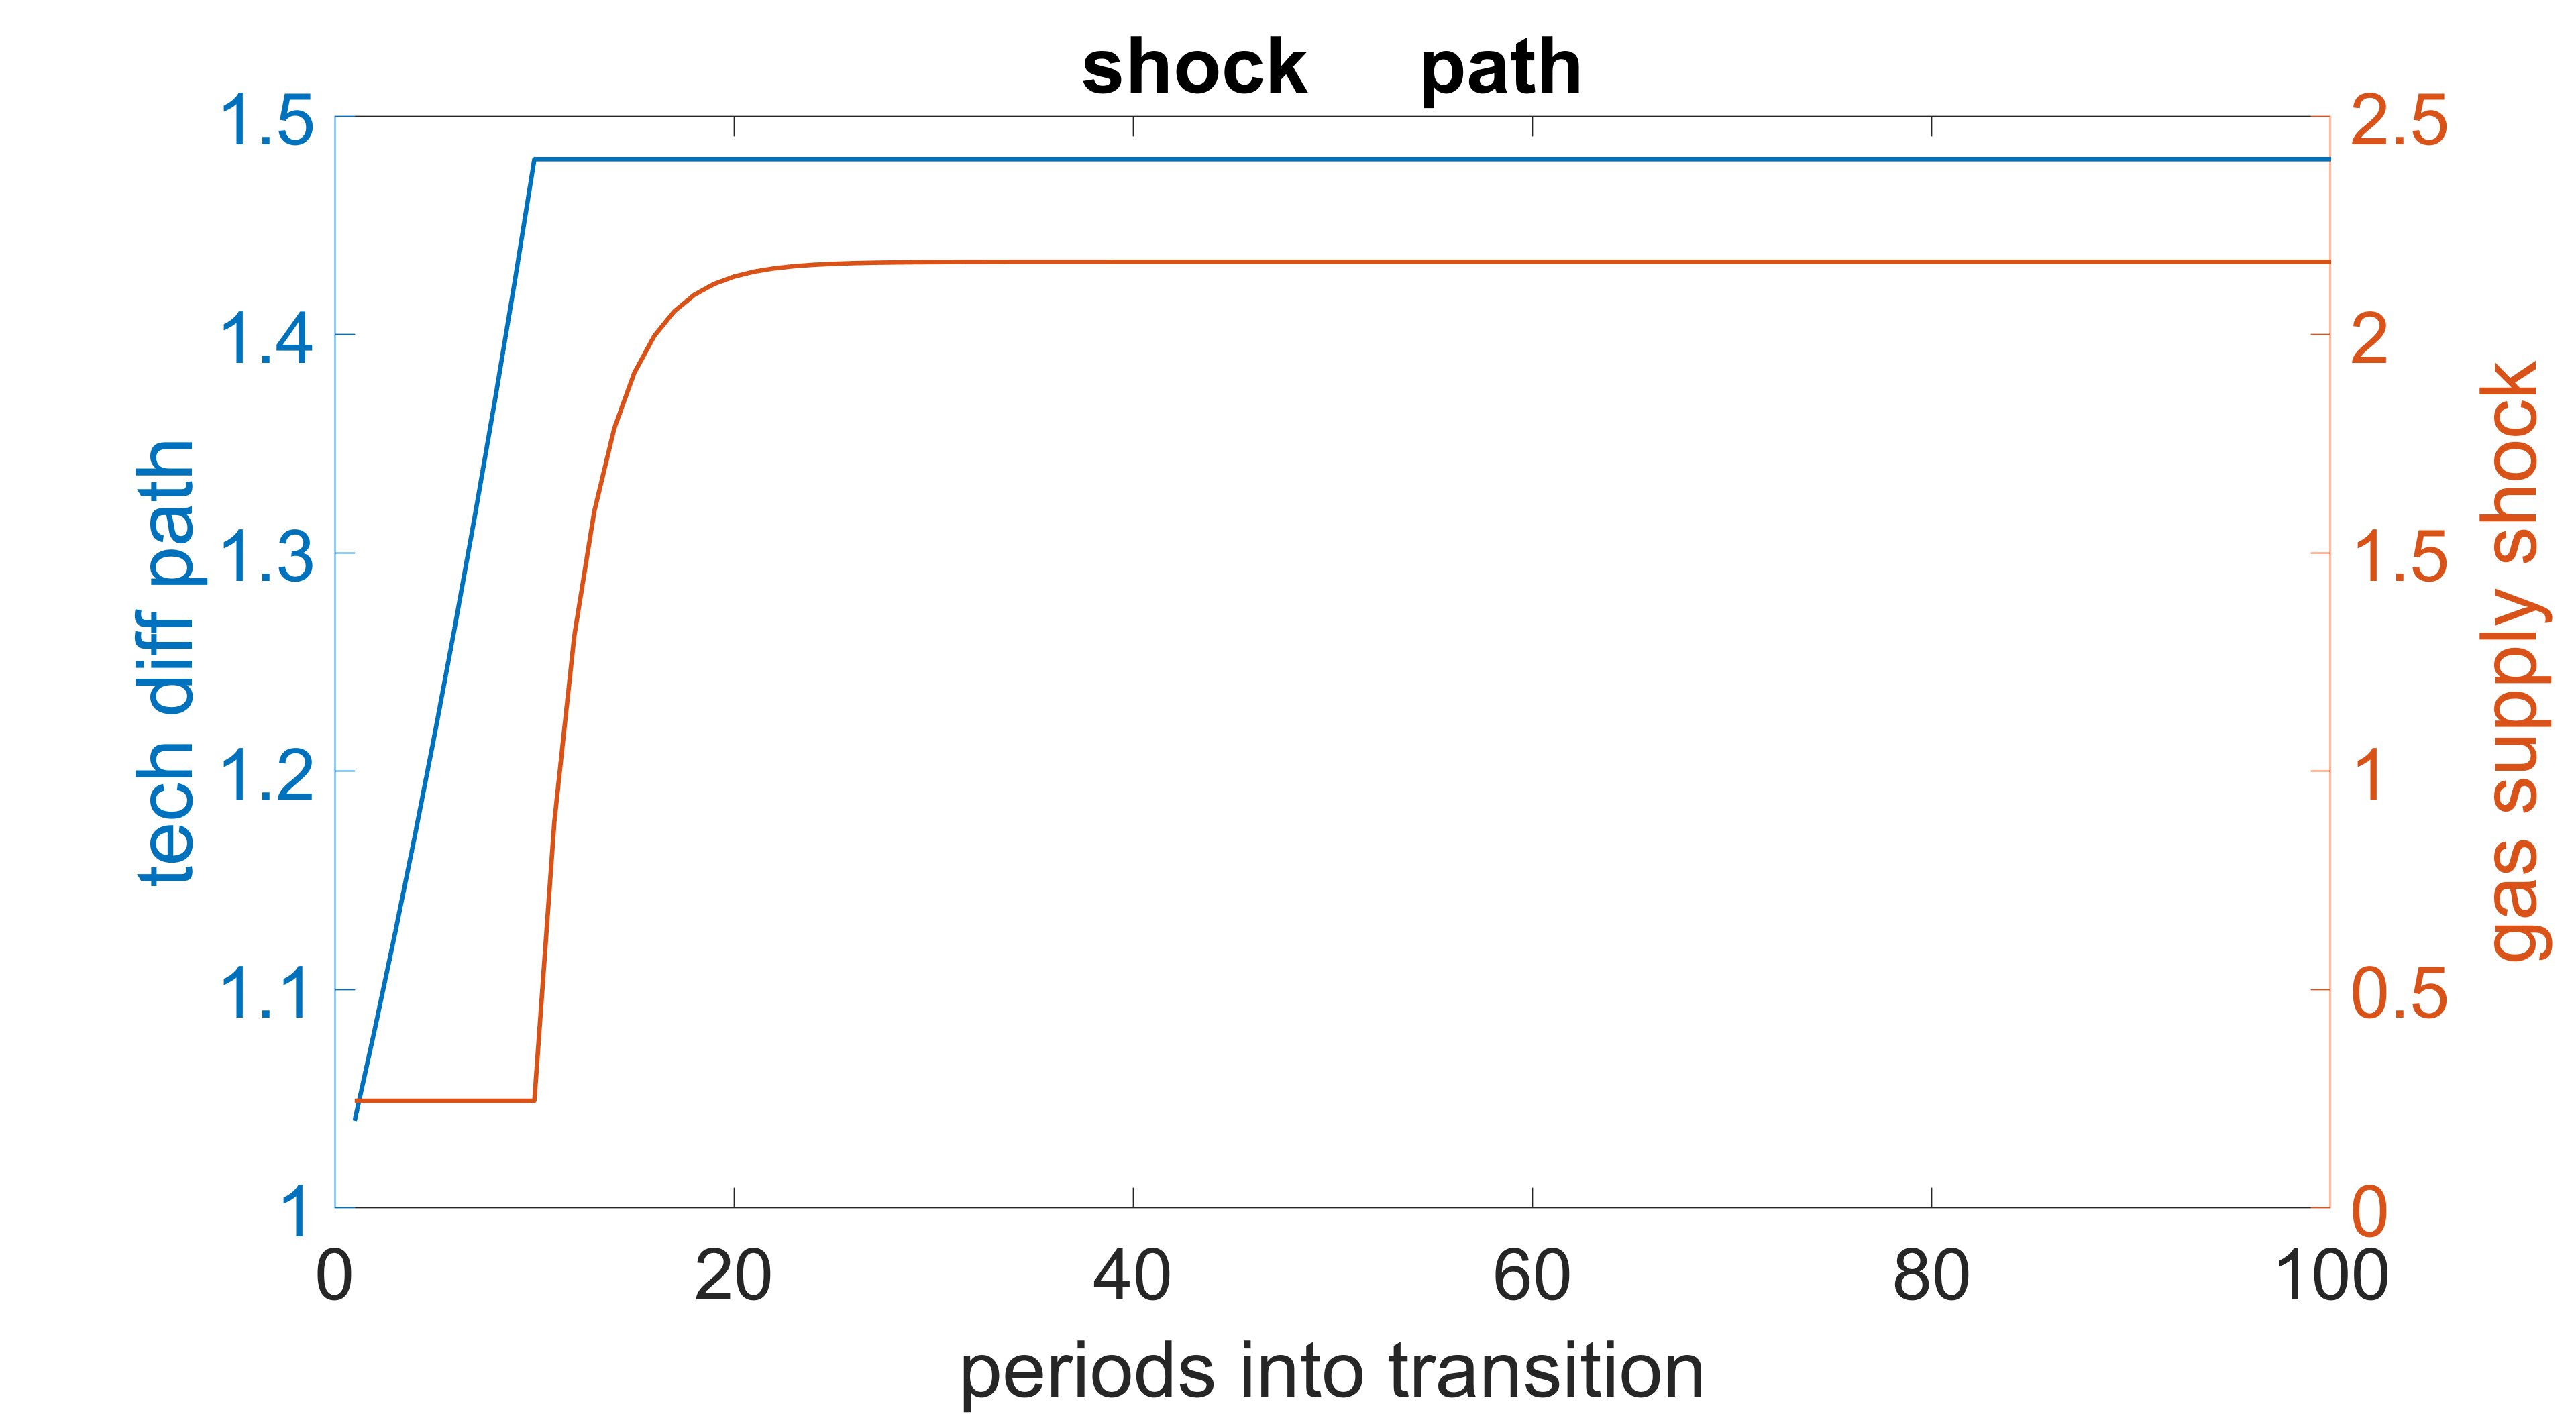
\includegraphics[scale=0.27]{shock path cg.png}
\end{figure}

\end{frame}
%%%%%%%%%%%%%%%
\begin{frame}{Transition 1: Conventional fuels to natural gas}
\begin{figure}
\centering
\caption{Share of solar and wind over the convergence path}
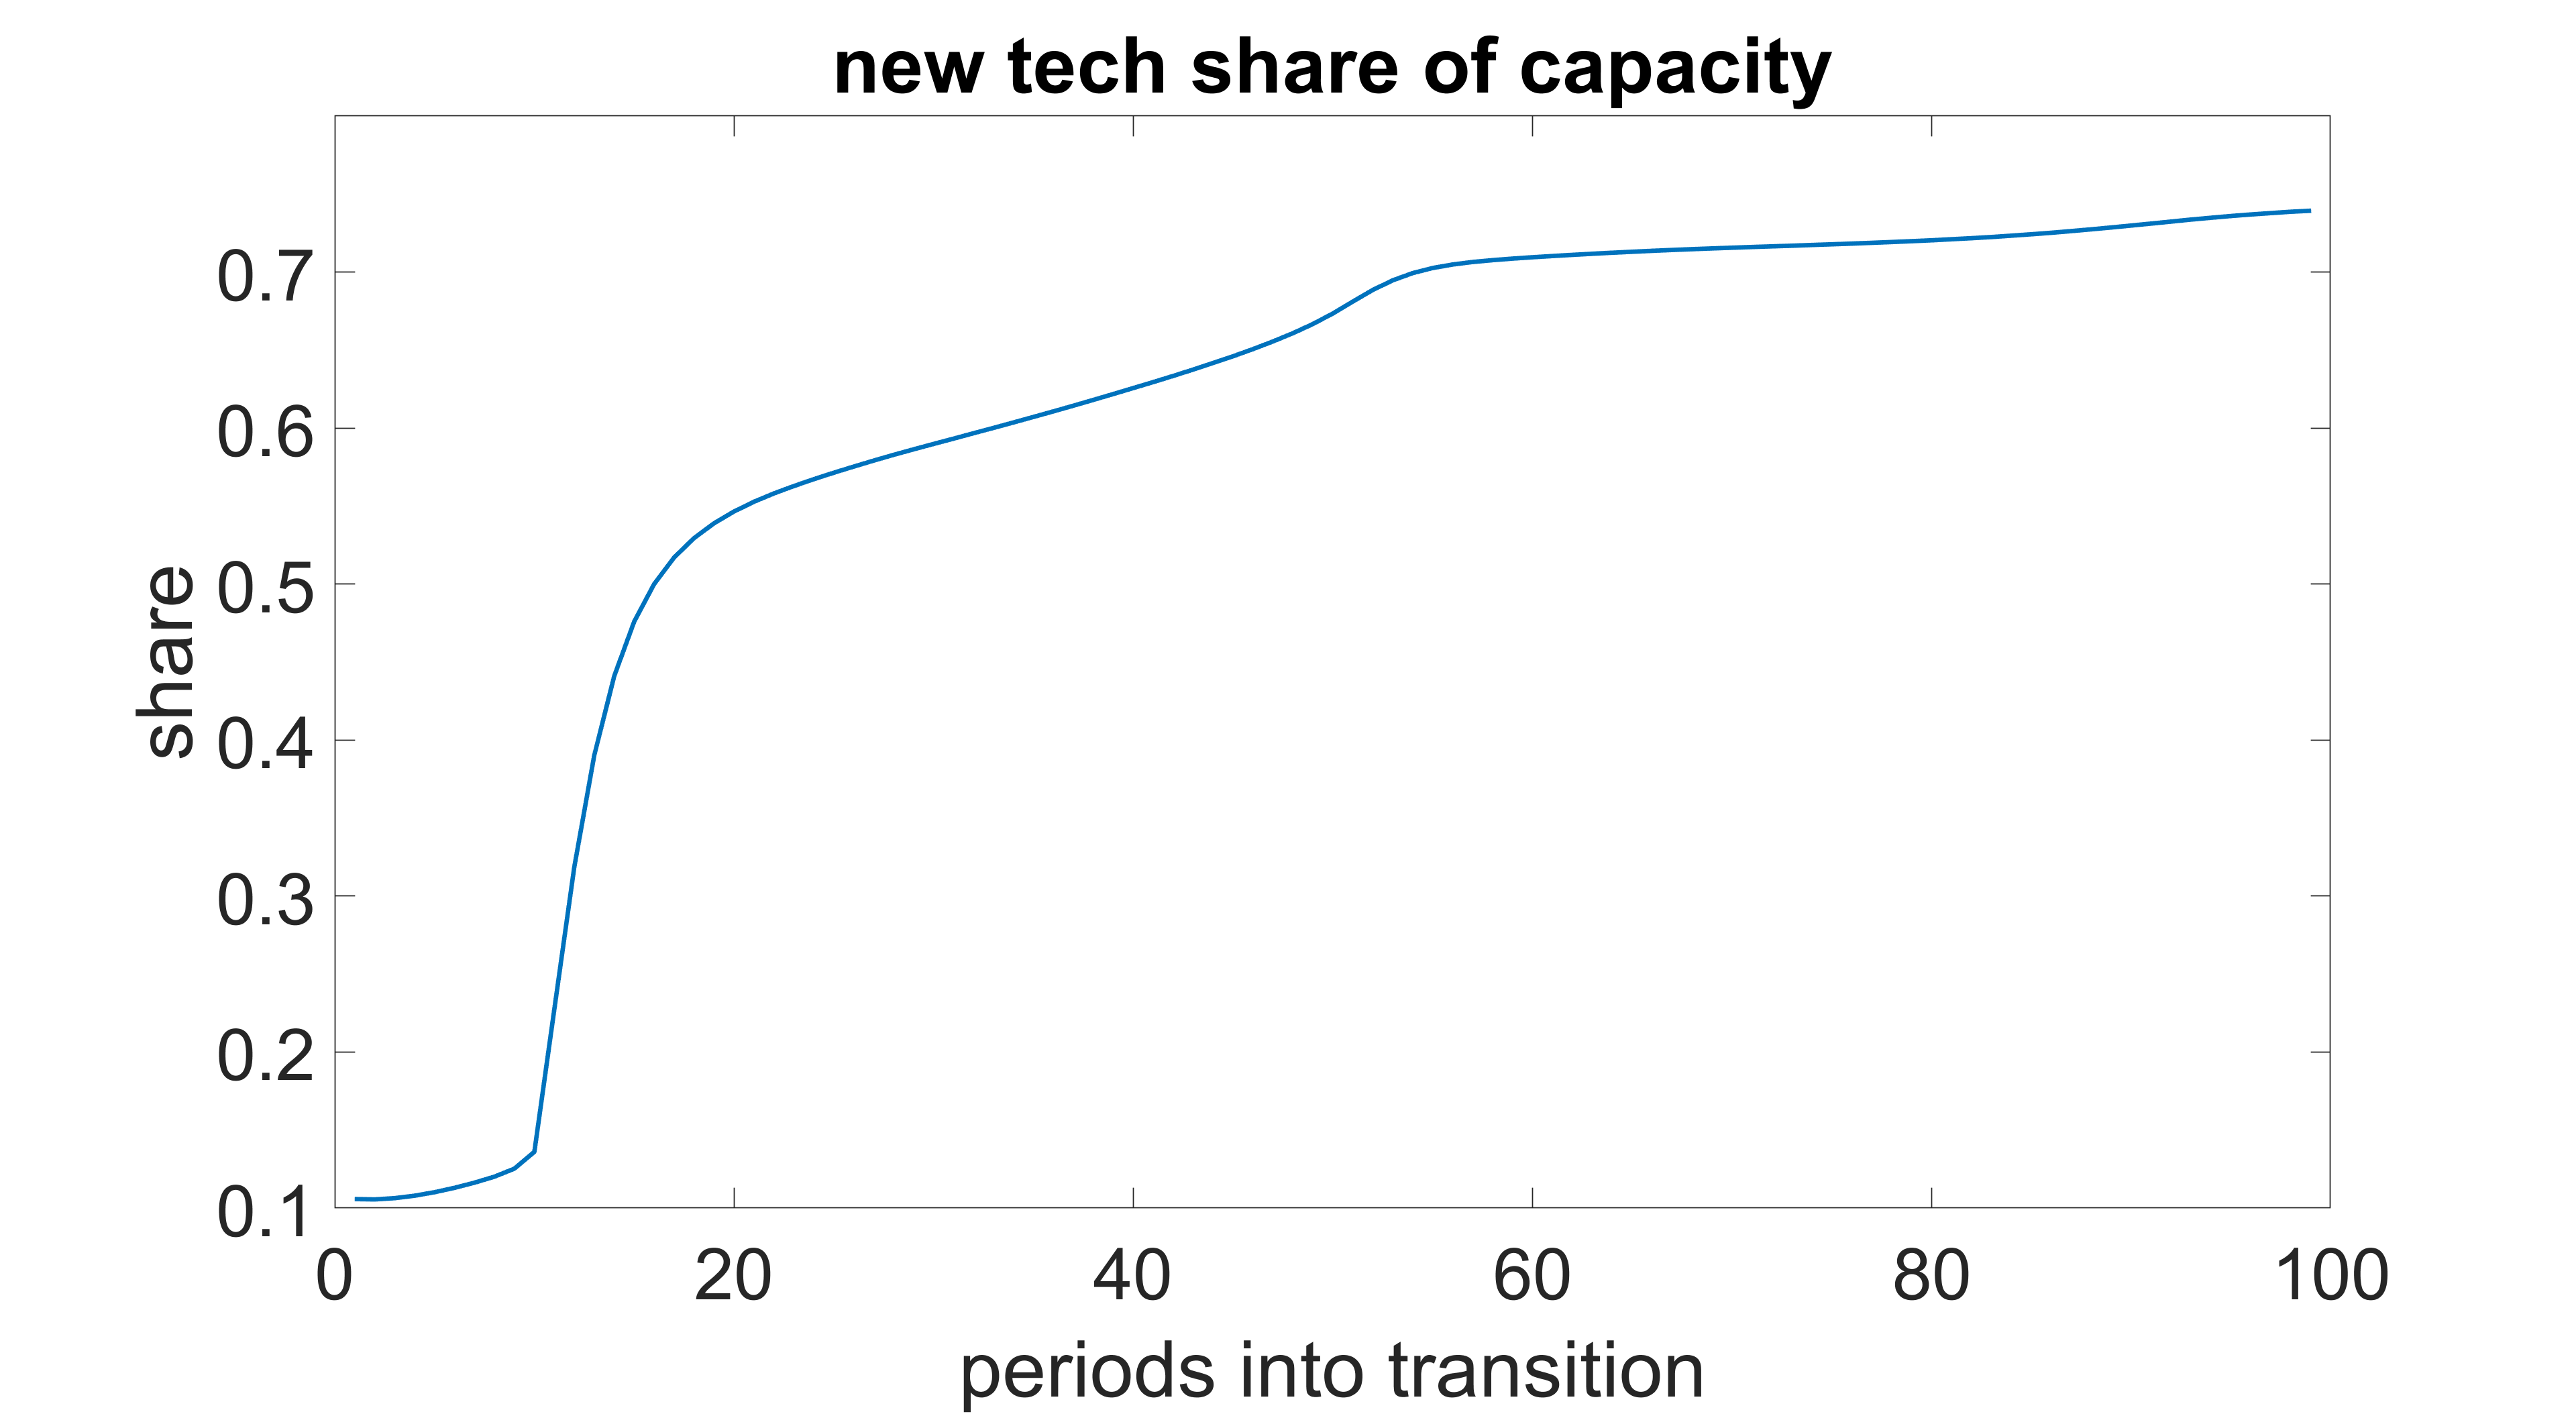
\includegraphics[scale=0.3]{share path.png}
\end{figure}

\end{frame}

%%%%%%%%%%%%%%%%%%%%%%%%%%%%%%%%%%%%%%%%%%%%%%%%%%%%%%%
\begin{frame}{Transition 1: Conventional fuels to natural gas}
\begin{figure}
\centering
\caption{Electricity price over the convergence path}
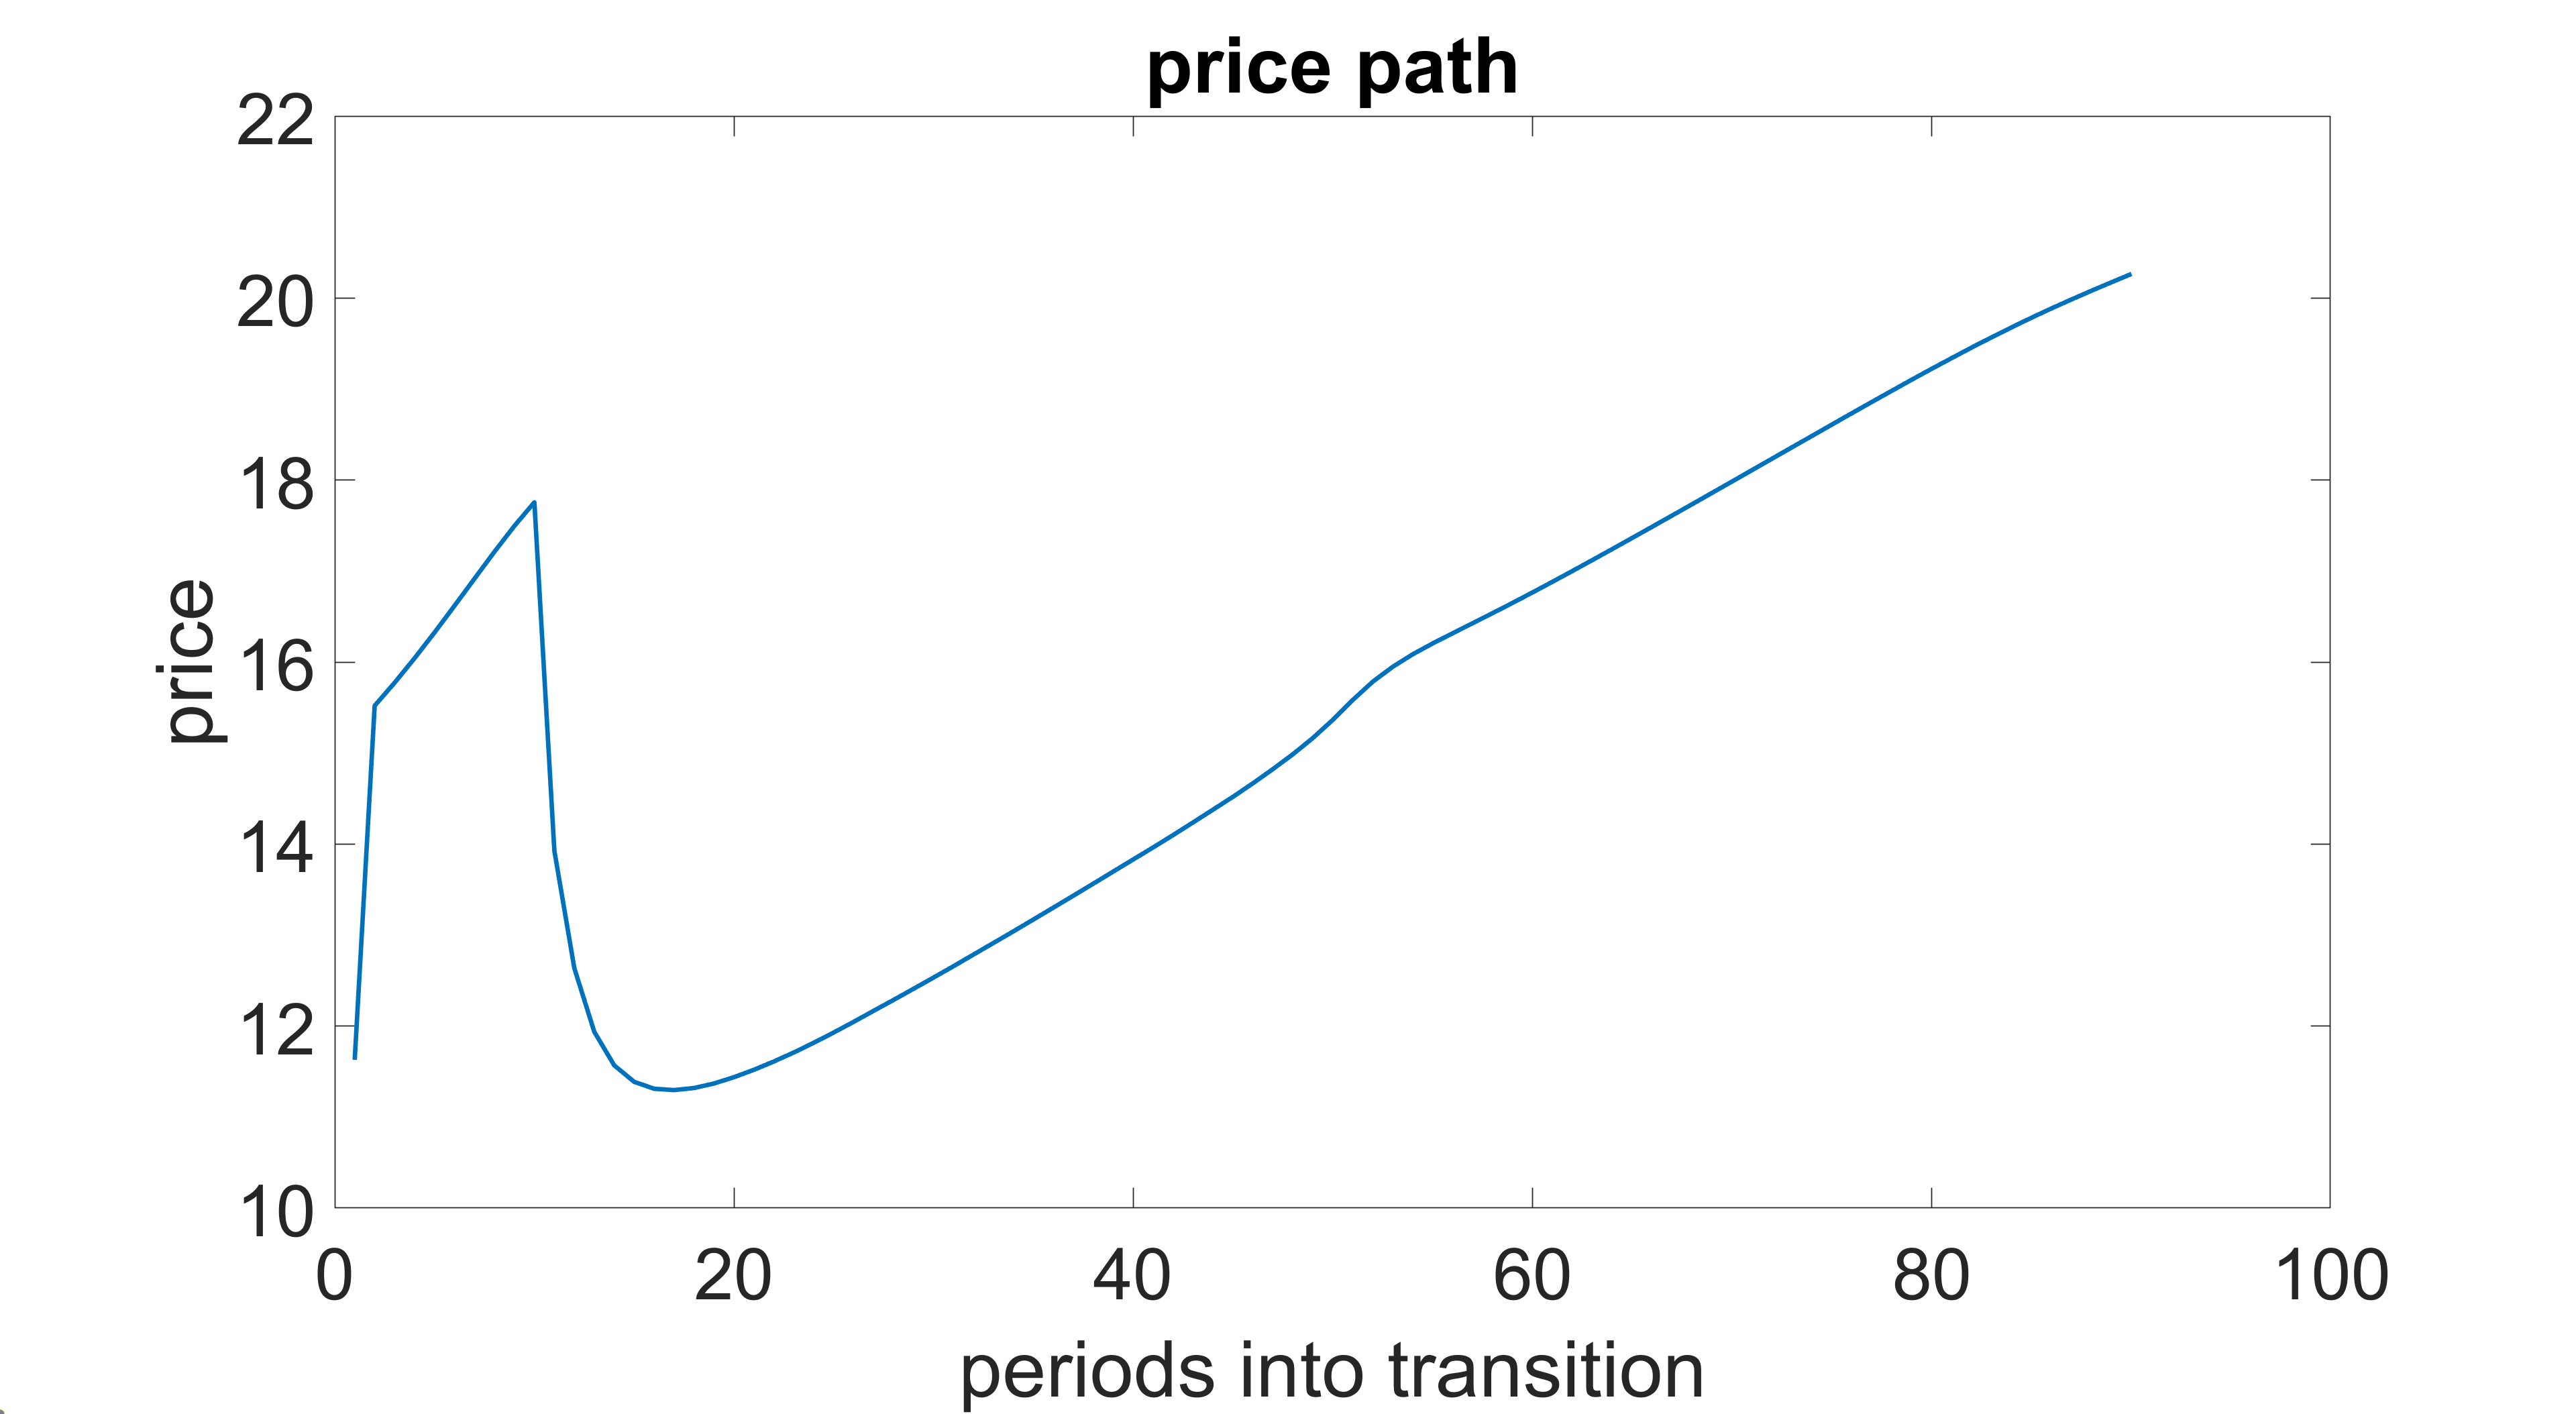
\includegraphics[scale=0.3]{price path.png}
\end{figure}

\end{frame}

%%%%%%%%%%%%%%%
\begin{frame}{Transition 2: Conventional fuels to solar and wind}

\begin{figure}
\centering
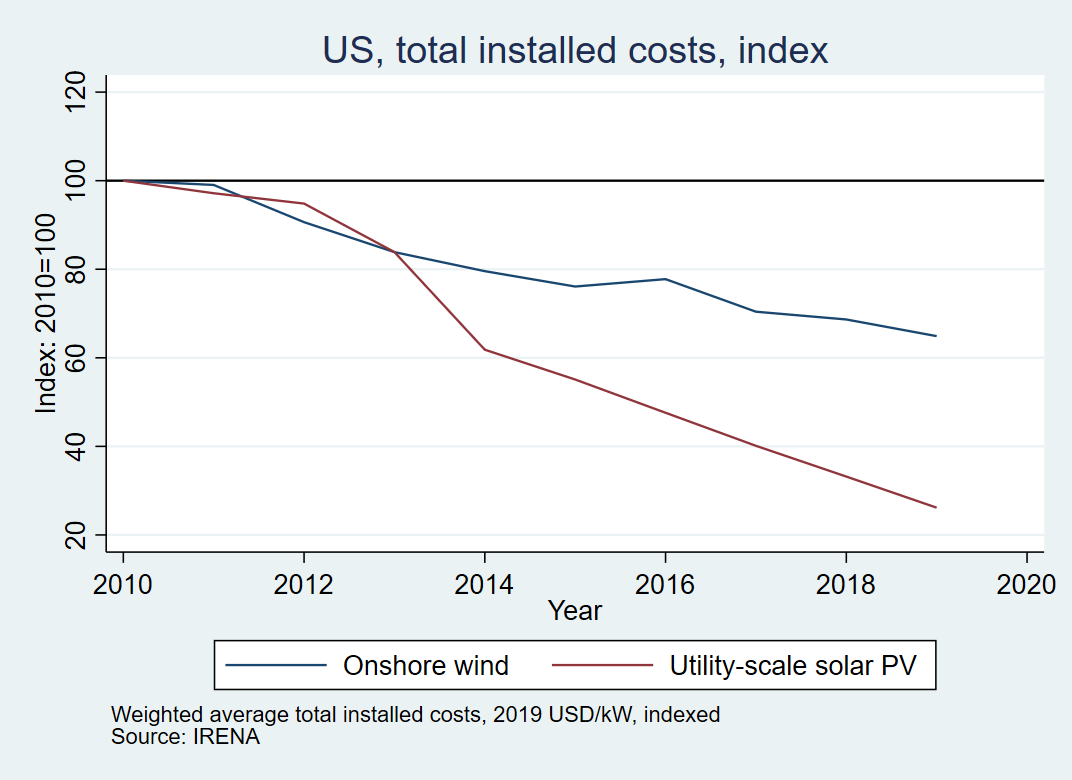
\includegraphics[scale=0.25]{solarwind_installedcosts_index.png}
\end{figure}

    
\end{frame}
%%%%%%%%%%%%%%%
\begin{frame}{Transition 2: Conventional fuels to solar and wind}

\begin{figure}
\centering
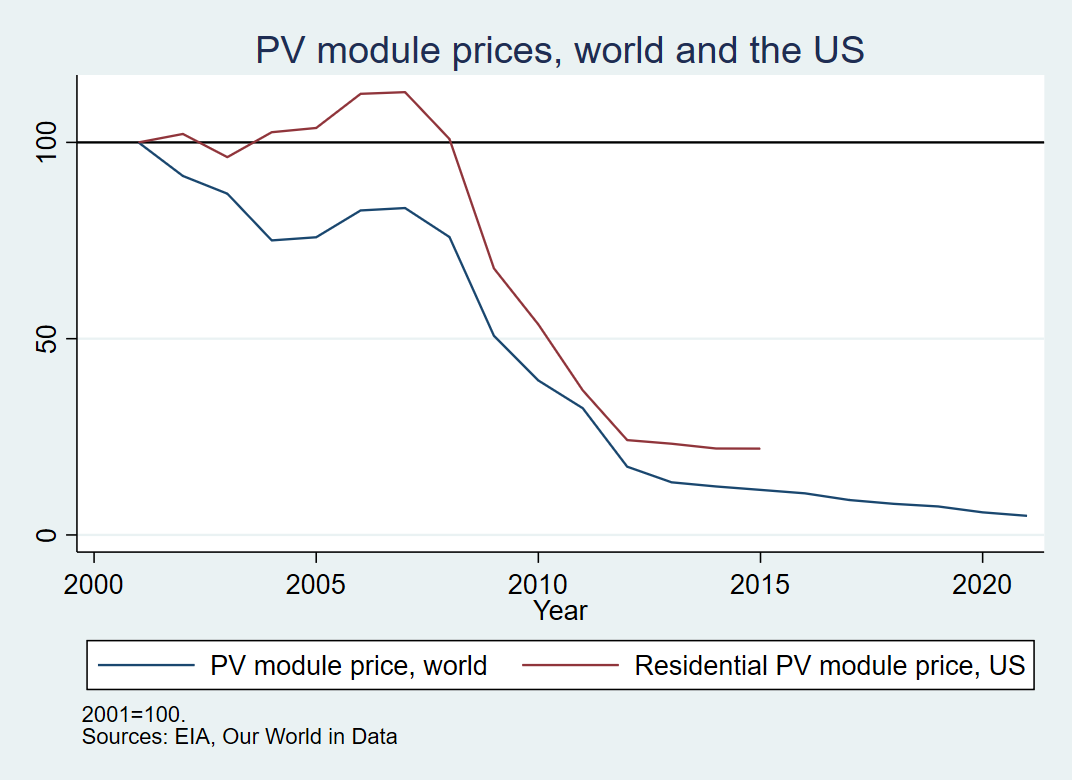
\includegraphics[scale=0.25]{solar_panelprice.png}
\end{figure}

    
\end{frame}
%%%%%%%%%%%%%%%
\begin{frame}{Transition 2: Conventional fuels to solar and wind}
\begin{figure}
\centering
\caption{The path of installation costs in the model}
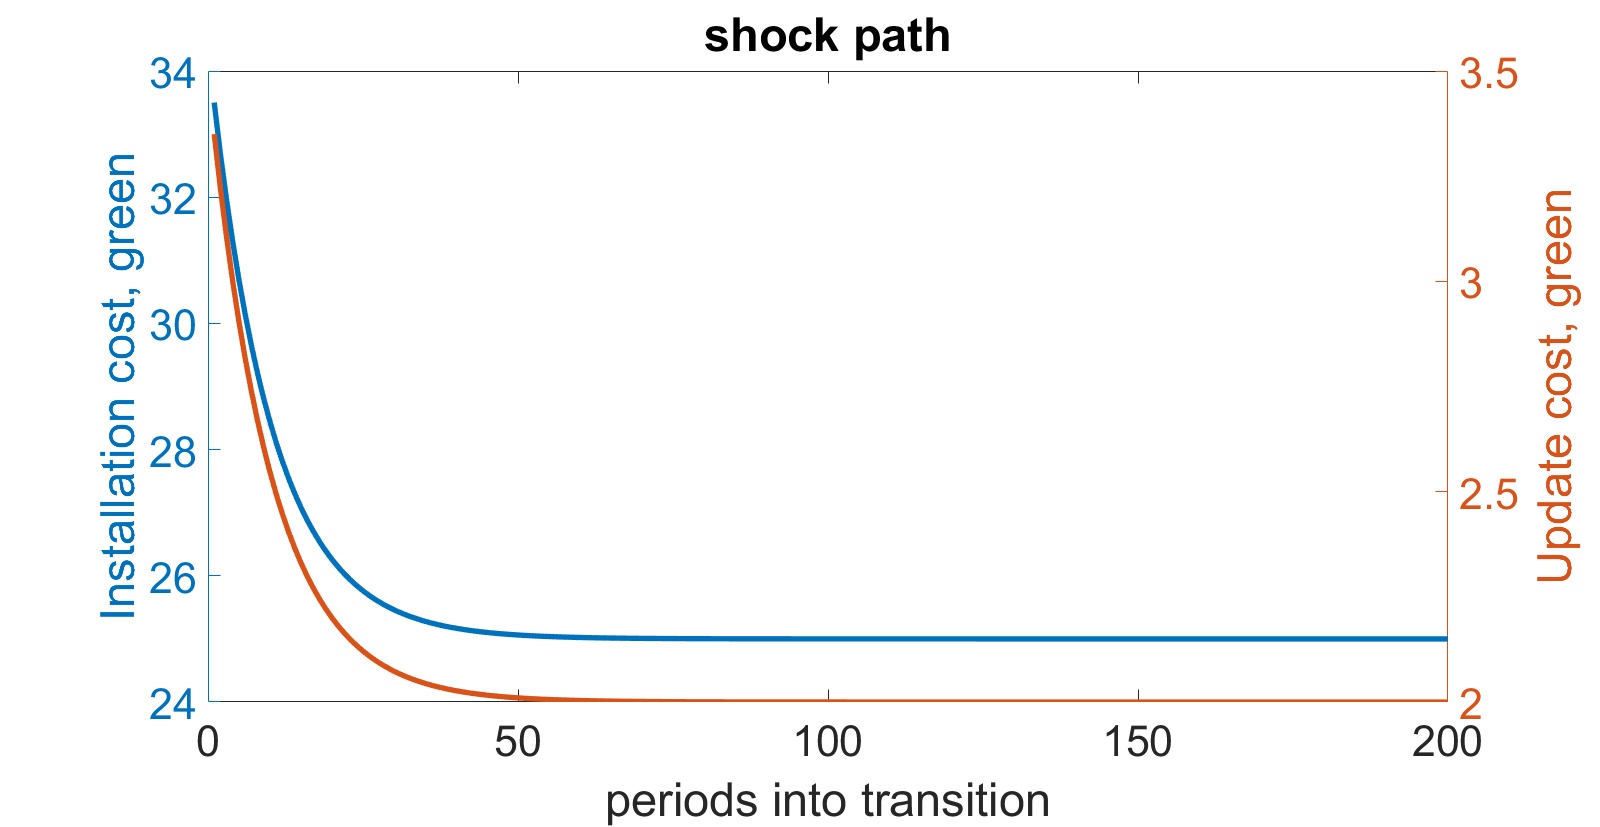
\includegraphics[scale=0.27]{shock path.png}
\end{figure}

\end{frame}
%%%%%%%%%%%%%%%
\begin{frame}{Transition 2: Conventional fuels to solar and wind}
\begin{figure}
\centering
\caption{Share of solar and wind over the convergence path}
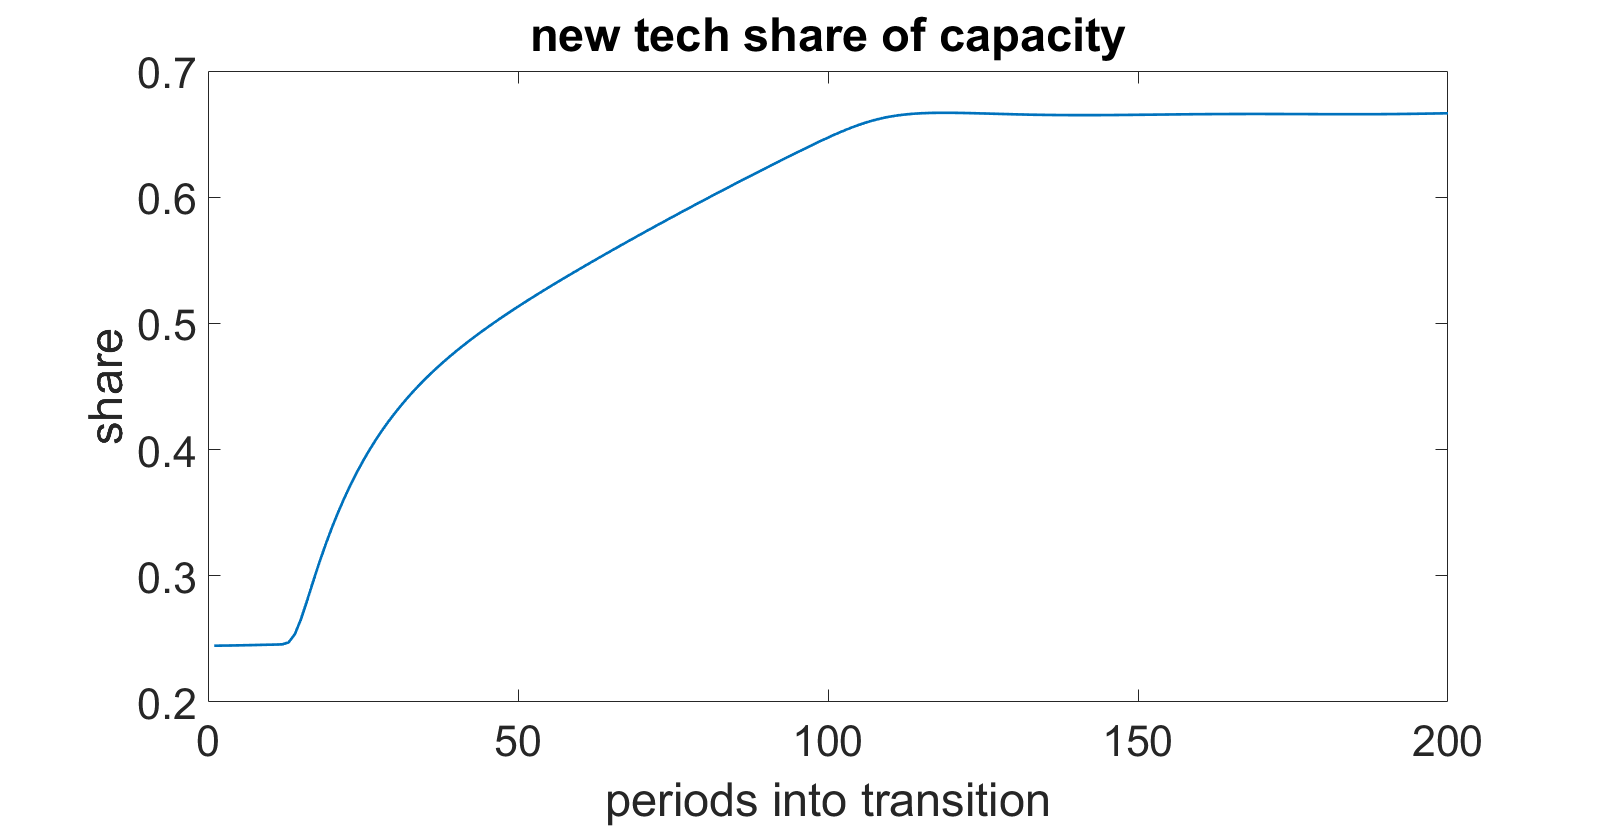
\includegraphics[scale=0.3]{share_path.png}
\end{figure}

\end{frame}

%%%%%%%%%%%%%%%%%%%%%%%%%%%%%%%%%%%%%%%%%%%%%%%%%%%%%%%
\begin{frame}{Transition 2: Conventional fuels to solar and wind}
\begin{figure}
\centering
\caption{Electricity price over the convergence path}
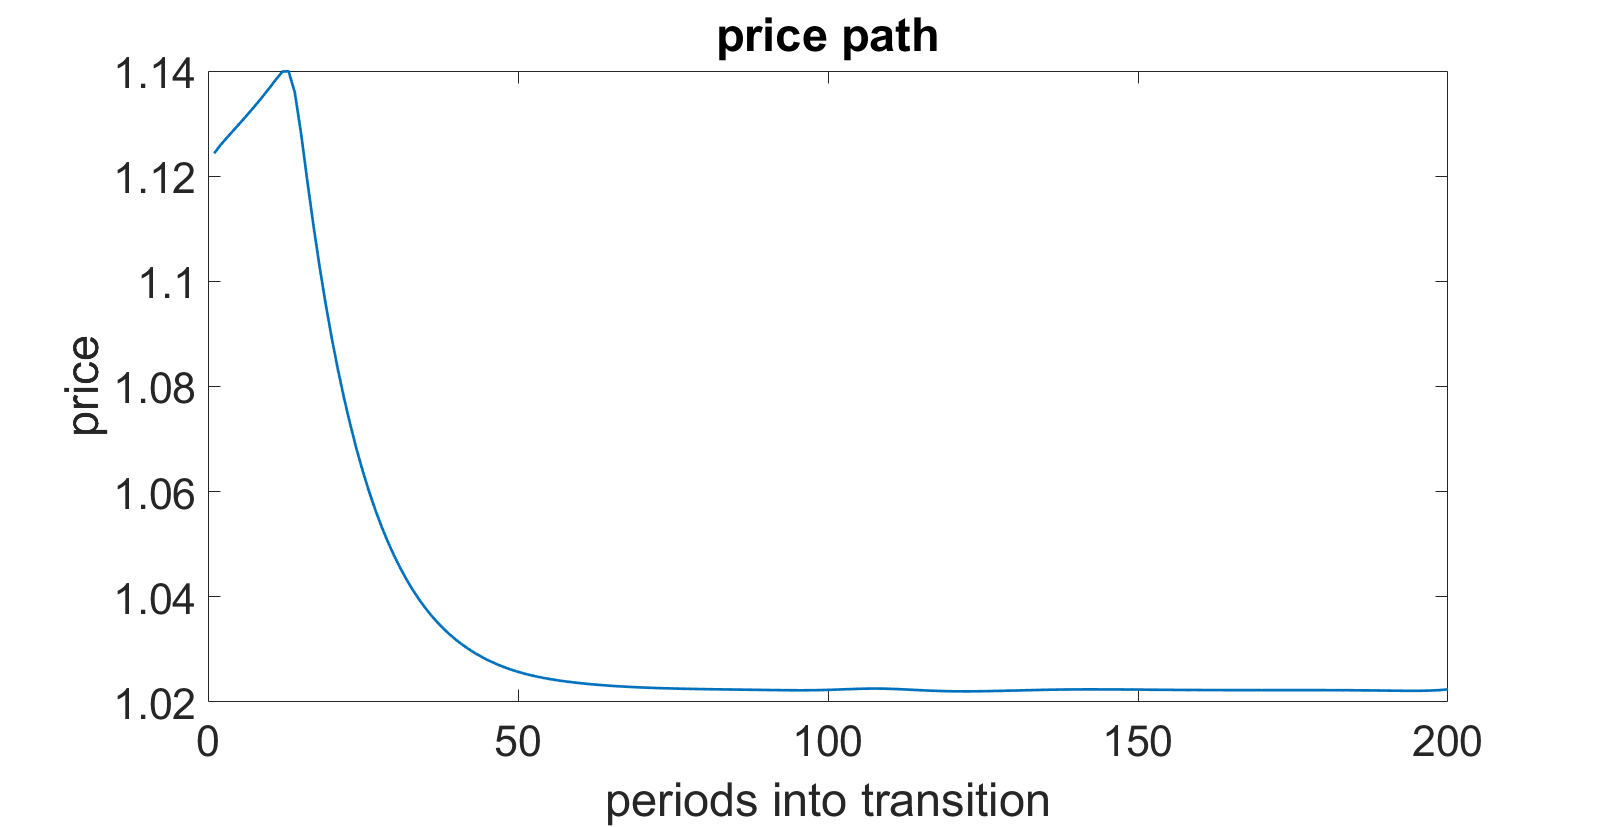
\includegraphics[scale=0.3]{price_path.png}
\end{figure}

\end{frame}

%%%%%%%%%%%%%%%%%%%%%%%%%%%%%%%%%%%%%%%%%%%%%%%%%%%%%%%
\begin{frame}{Appendix}


\end{frame}

%%%%%%%%%%%%%%%
%%%%%%%%%%%%%%%
\begin{frame}{Intra-period problem}
    From the intra-period optimization of the generators we would have:\\
    \begin{align*}
        e_i^* = (\frac{a_{i,t}p_E\alpha}{p_e})^\frac{1}{1-\alpha}
    \end{align*}
    In the data $\a_{i,t}$ would be the relative efficiency of the generator. The reason for doing so is that from the generator's perspective whether its own efficiency depreciates or others' efficiency grow with rate $1+g$  (and market base demand with rate $(1+g)^\frac{1}{1-\alpha}$) it would face a similar problem. Therefore we consider the effects of both the growth of other techs and own depreciation as one depreciation effect
\end{frame}
%%%%%%%%%%%%%%%
%%%%%%%%%%%%%%%
\begin{frame}{Alternative model setup}
\small Since we're considering the total generation of a unit in one period (year) we can also consider the production function of a generator as a CRS function however the average price that a generator observes would reduce as it increases its active time (input in the model). This happens since when a generator decides to be active for a short amount of time in a year it can choose the active time optimally over the day to supply during the peak times with the highest price. Since we don't consider the daily variations of the electricity price in our model it means that when the input is low the generator would see an average price higher than the average yearly price since it can allocate its determined generation to the slots with higher prices. As it decides to put more input into generation it will have to choose slots with lower prices to supply its electricity to the market. Lets say for the average price that the generator observes we have:
    \small\begin{align*}
        p_E(e_i) = p_0e_i^{-\eta}
    \end{align*}
    \small Then for the intra-period problem it solve:
    \small\begin{align*}
        \max_{e_i} a_{i,t}e_ip_E(e_i) - p_ee_i \rightarrow e_i^* = (\frac{p_0a_{i,t}(1-\eta)}{p_e})^\frac{1}{\eta} \\\rightarrow \alpha = 1-\eta , p_E = p_0\frac{\eta}{1-\eta} \text{ equalizes the two settings}
    \end{align*}
\end{frame}
\begin{frame}{Summary statistics, smaller sample}
\input{summarystats_inpart4_10_5_all_sameN_small}
\footnotesize{Note: Adoption dummy defined as efficiency increase of at least 10\% with less than 5\% variation in the capacity-to-generation dummy }
    
\end{frame}
%%%%%%%%%%%%%%%
\begin{frame}{Summary statistics, single-generator plants}
\begin{table}[htbp]\centering
\footnotesize
\def\sym#1{\ifmmode^{#1}\else\(^{#1}\)\fi}
\caption{Summary statistics, Single-generator plants used in analysis}
\begin{tabular}{l*{1}{ccccc}}
\hline\hline
                    &        mean&          sd&         min&         max&           N\\
\hline
No of generators    &         1.0&         0.0&         1.0&         1.0&       2,517\\
No of energy sources used&         1.0&         0.0&         1.0&         1.0&       2,517\\
No of energy sources per generator&         1.4&         0.8&         1.0&         6.0&       2,517\\
Average generator age&        13.8&        12.8&         0.0&        64.0&       2,517\\
Summer capacity     &        88.0&       205.9&         0.1&     1,344.0&       2,517\\
Fuel efficiency     &         0.3&         0.1&         0.0&         0.9&       2,475\\
Relative efficiency &         0.9&         0.4&         0.0&         2.8&       2,475\\
Relative efficiency after latest upgrade&         1.0&         0.4&         0.0&         3.3&       2,489\\
Share updating per year&         2.0&        14.1&         0.0&       100.0&       2,454\\
Share updating per year, unconstrained&        12.4&        33.0&         0.0&       100.0&       2,454\\
\hline\hline
\multicolumn{6}{l}{\footnotesize Note: Summary statistics over plant-year}\\
\end{tabular}
\end{table}

\footnotesize{Note: Adoption dummy defined as efficiency increase of at least 10\% with less than 5\% variation in the capacity-tp-generation dummy }
    
\end{frame}
%%%%%%%%%%%%%%%
\begin{frame}{Data, part4: Adoption likelihood and efficiency}

\begin{figure}
\centering
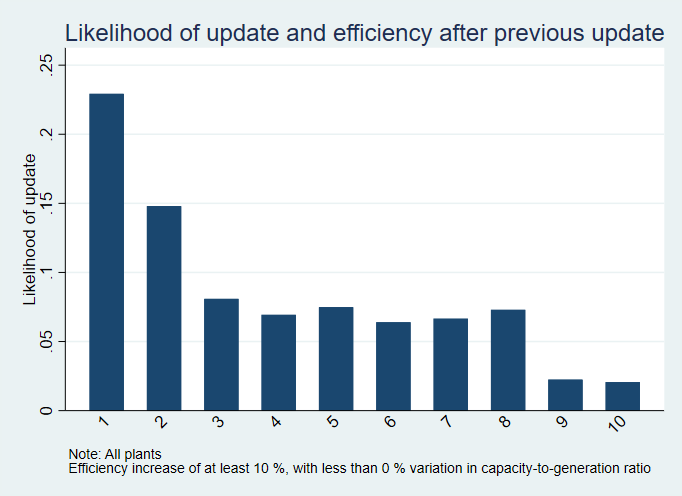
\includegraphics[scale=0.25]{hist_effic_updatedummy_all.png}
\end{figure}

    
\end{frame}
%%%%%%%%%%%%%%%
\begin{frame}{Data, part 4: Adoption likelihood and capacity age}

\begin{figure}
\centering
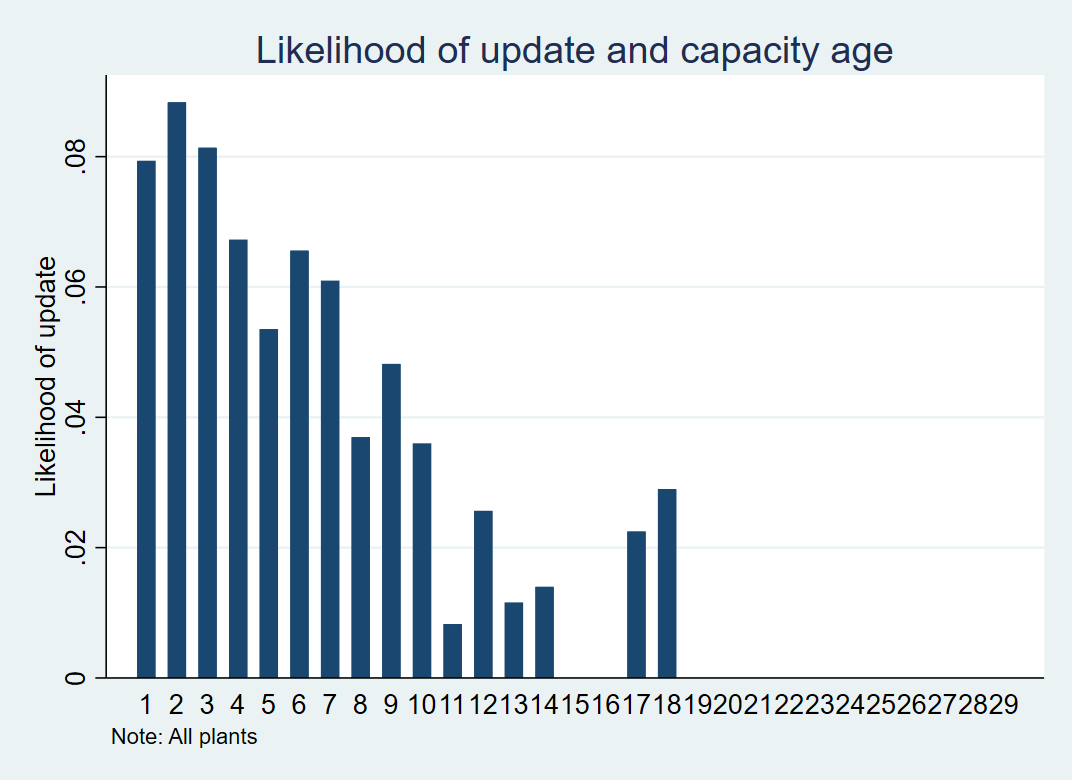
\includegraphics[scale=0.25]{hist_capage_updatedummy_all.png}
\end{figure}

    
\end{frame}
%%%%%%%%%%%%%%%


\begin{frame}{Data, part 4: Efficiency and capacity age}

\begin{figure}
\centering
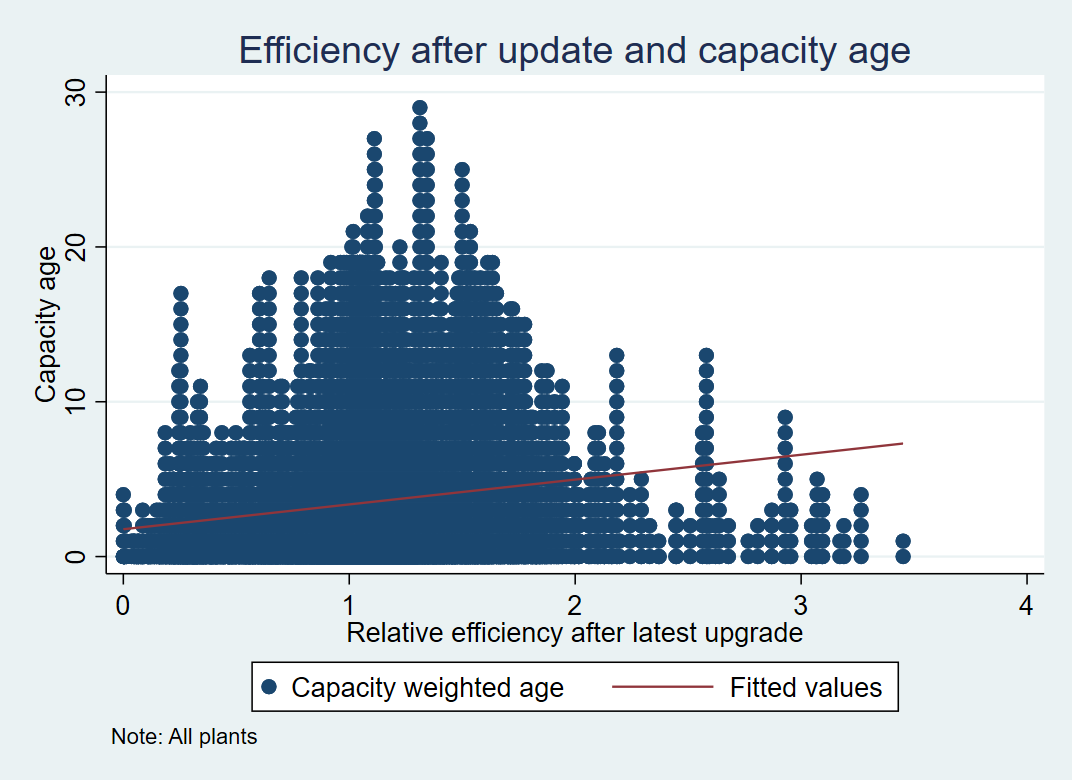
\includegraphics[scale=0.25]{scatter_effic_capage_all.png}
\end{figure}

    
\end{frame}
%%%%%%%%%%%%%%%
\begin{frame}{Results for calibration: Efficiency in periods between updates and capacity age}

\begin{figure}
\centering
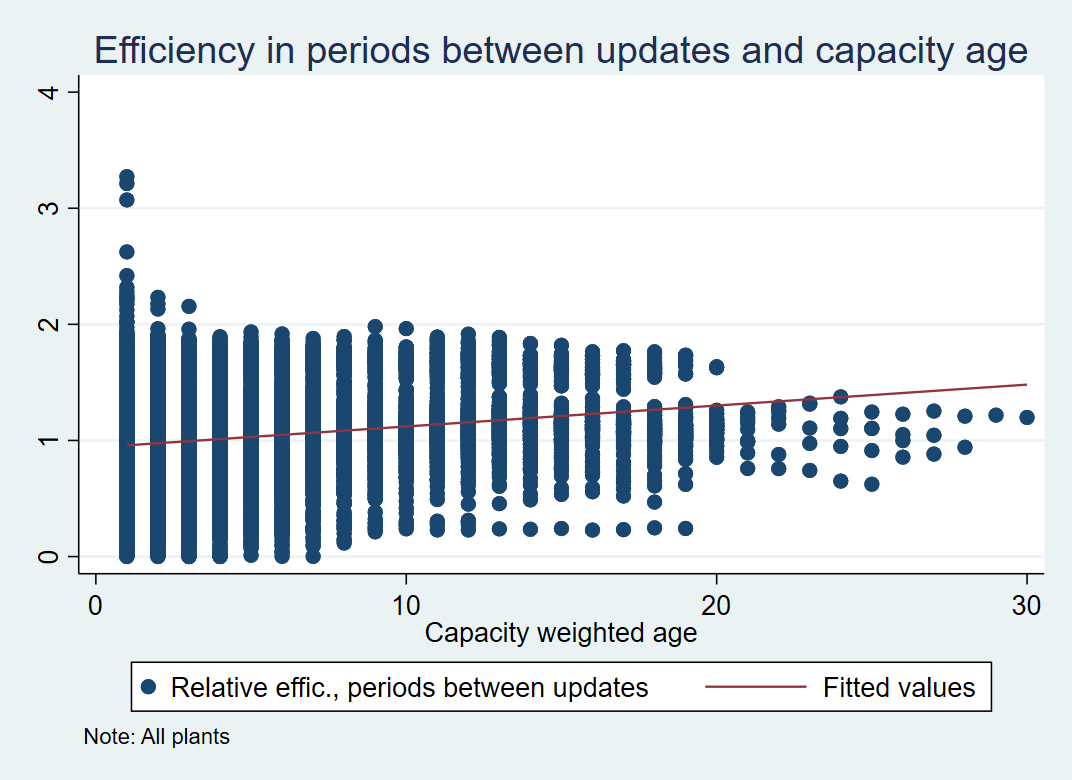
\includegraphics[scale=0.25]{5_scatter_effic_noupd_capage_all.png}
\end{figure}

\end{frame}

%%%%%%%%%%%%%%%
\begin{frame}{Results for calibration: Efficiency in periods between updates and after latest update}

\begin{figure}
\centering
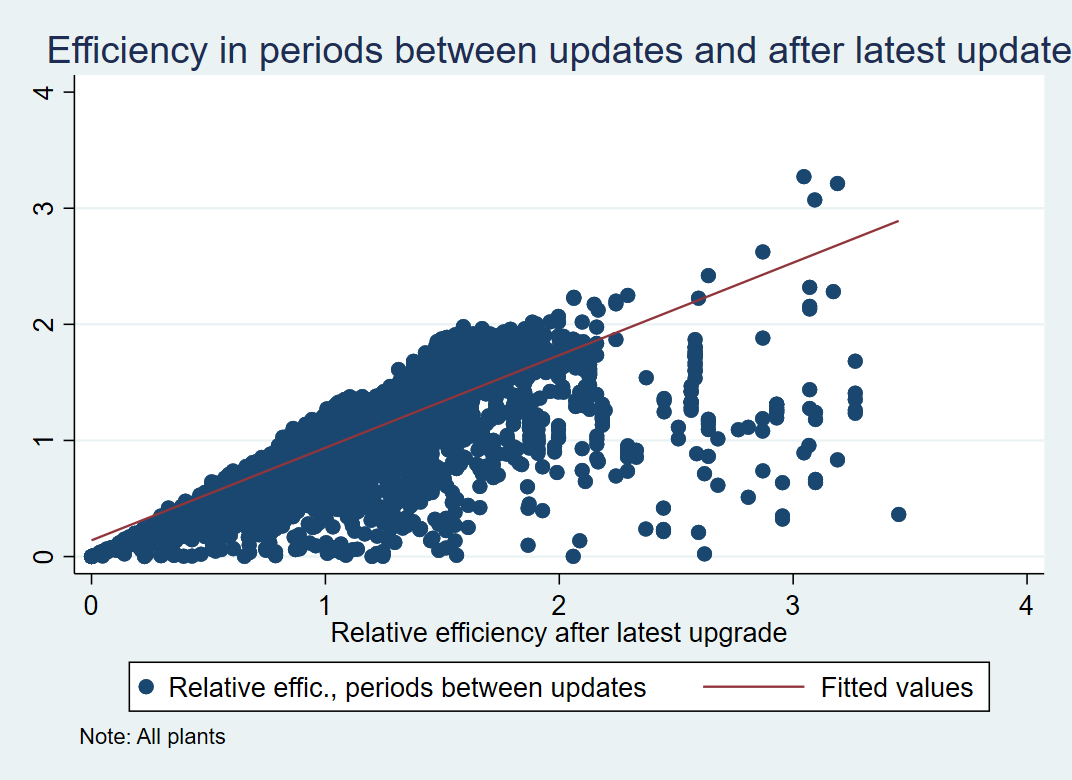
\includegraphics[scale=0.25]{5_scatter_effic_noupd_effic_new_all.png}
\end{figure}

\end{frame}

%%%%%%%%%%%%%%%
\begin{frame}{Results for calibration: Efficiency in periods between updates and plant average capacity age}

\begin{figure}
\centering
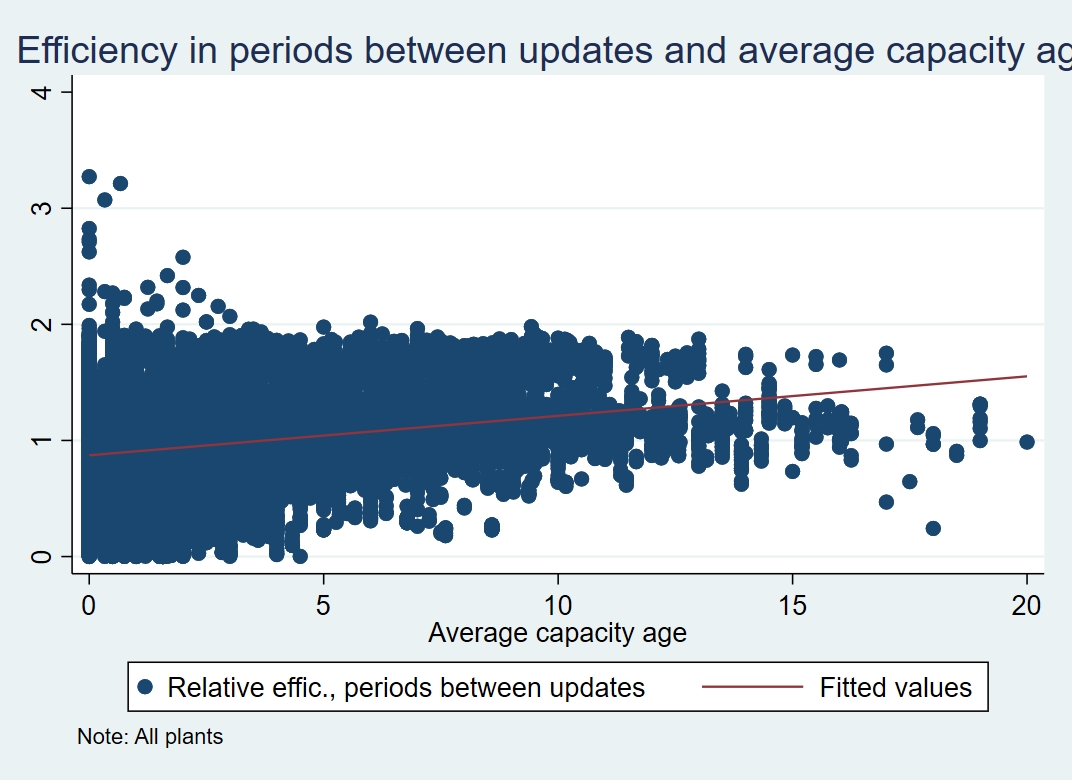
\includegraphics[scale=0.25]{5_scatter_effic_noupd_durab2_all.png}
\end{figure}

\end{frame}

%%%%%%%%%%%%%%%
\begin{frame}{Results for calibration: Efficiency after latest update and plant average capacity age}

\begin{figure}
\centering
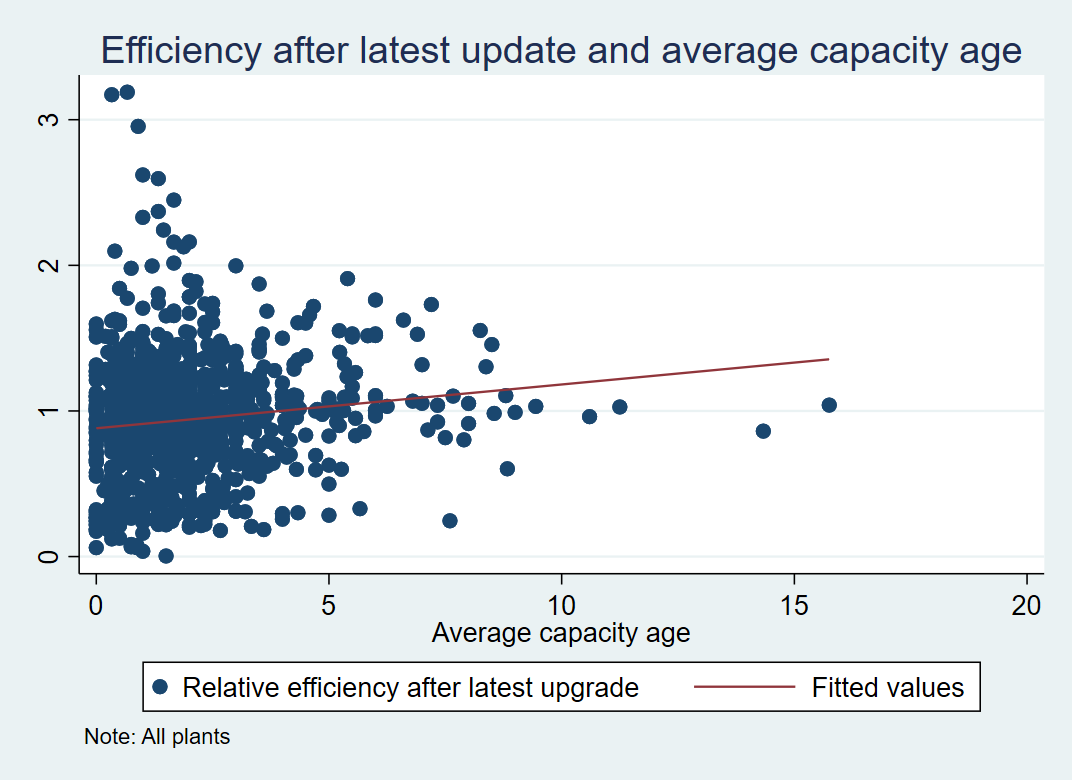
\includegraphics[scale=0.25]{5_scatter_effic_new_durab2_all.png}
\end{figure}

\end{frame}

%%%%%%%%%%%%%%%


\end{document}

